\documentclass[a4paper,11pt]{article}
\pdfoutput=1 
\usepackage{jheppub} 
\usepackage[numbers]{natbib}
\usepackage[T1]{fontenc} 
\usepackage[compat=1.1.0]{tikz-feynman}
\usepackage{xcolor}
\usepackage{multirow}
\usepackage{multicol}
\usepackage{float}
\usepackage{verbatim,slashed}
\usepackage{amsmath,mathtools}
\usepackage{relsize,float}
\usepackage{bm, nicefrac}
\usepackage{hyperref}
\usepackage[capitalise]{cleveref}
\usepackage{comment}
\usepackage{booktabs}
\usepackage[normalem]{ulem}
\usepackage{overpic}

\newcommand{\pdp}{\ensuremath{\phi^\dagger\phi}}
\renewcommand{\phi}{\ensuremath{\varphi}}
\newcommand{\sss}{\scriptscriptstyle}
\newcommand{\sst}{\scriptstyle}
\newcommand{\OO}{\ensuremath{\mathcal{O}}}
\newcommand{\QQ}{\ensuremath{\mathcal{Q}}}
\newcommand{\Op}[1]{\OO_{\sss #1}}
\newcommand{\Opp}[2]{\OO_{\sss #1}^{\sss #2}}
\newcommand{\Oppd}[2]{^{\dagger}\OO_{\sss #1}^{\sss #2}}
\newcommand{\Qp}[1]{\QQ_{\sss #1}}
\newcommand{\Qpp}[2]{\QQ_{\sss #1}^{\sss #2}}
\newcommand{\Qppd}[2]{^{\dagger}\QQ_{\sss #1}^{\sss #2}}
\newcommand{\lam}{\Lambda}
\newcommand{\cp}[1]{c_{\sss #1}}
\newcommand{\Cp}[1]{C_{\sss #1}}
\newcommand{\cpp}[2]{c_{\sss #1}^{\sss #2}}
\newcommand{\Cpp}[2]{C_{\sss #1}^{\sss #2}}
\def\lra#1{\overset{\text{\scriptsize$\leftrightarrow$}}{#1}}
%\newcommand{\sw}{s_{\sss W}}
%\newcommand{\cw}{c_{\sss W}}
\newcommand{\mw}{m_{\sss W}}
\newcommand{\mz}{m_{\sss Z}}
\newcommand{\mt}{m_{t}}
\newcommand{\ttbar}{t\bar{t}}
\newcommand{\ttZ}{t\bar{t}Z}
\newcommand{\mwz}{m_{\sss WZ}}
\newcommand{\gztr}{g^{\sss Z}_{t_{\sss R}}}
\newcommand{\gztl}{g^{\sss Z}_{t_{\sss L}}}
\newcommand{\gzbr}{g^{\sss Z}_{b_{\sss R}}}
\newcommand{\gzbl}{g^{\sss Z}_{b_{\sss L}}}
\newcommand{\gbtw}{g_{\sss btW}}
\newcommand{\gta}{g_{\sss t\gamma}}
\newcommand{\gwa}{g_{\sss W\gamma}}
\newcommand{\gwz}{g_{\sss WZ}}
\newcommand{\dimreg}{dimensional regularisation}
\newcommand{\hv}{'t Hooft-Veltman }

\newcommand{\SDKweak}{Sudakov$_\text{weak}$ }

\newcommand{\OctTr}{$\Opp{Qq}{3,8}$}
\newcommand{\OctSi}{$\Opp{Qq}{1,8}$}
\newcommand{\QuOct}{$\Opp{Qu}{8}$}
\newcommand{\tqOct}{$\Opp{tq}{8}$}
\newcommand{\QdOct}{$\Opp{Qd}{8}$}
\newcommand{\tuOct}{$\Opp{tu}{8}$}
\newcommand{\tdOct}{$\Opp{td}{8}$}
\newcommand{\TriSi}{$\Opp{Qq}{3,1}$}
\newcommand{\SiSi}{$\Opp{Qq}{1,1}$}
\newcommand{\QuSi}{$\Opp{Qu}{1}$}
\newcommand{\tqSi}{$\Opp{tq}{1}$}
\newcommand{\QdSi}{$\Opp{Qd}{1}$}
\newcommand{\tuSi}{$\Opp{tu}{1}$}
\newcommand{\tdSi}{$\Opp{td}{1}$}
\newcommand{\QQSi}{$\Opp{QQ}{1}$}
\newcommand{\QQOct}{$\Opp{QQ}{8}$}
\newcommand{\ttSi}{$\Opp{tt}{1}$}
\newcommand{\QtSi}{$\Opp{Qt}{1}$}
\newcommand{\QtOct}{$\Opp{Qt}{8}$}

%%%%%%%%%%%
\renewcommand\arraystretch{1.1}
%\setlength{\textfloatsep}{10pt plus 1.0pt minus 2.0pt}

%NOTE: \beq and \eeq will not work if using amsmath. 
%Use \beqn and \eeqn instead
\def\beq{\begin{equation}}
\def\eeq{\end{equation}}
\def\beqn{\begin{eqnarray}}
\def\eeqn{\end{eqnarray}}
\def\abs#1{\left|#1\right|}
\def\IN{{\small IN}}
\def\OUT{{\small OUT}}
\def\remove#1#2{#1\hspace{-#2truecm}\backslash}
\def\removeb#1#2#3{#1\hspace{-#2truecm}\backslash\hspace{-#3truecm}\slash}
\def\red{}
\def\xidistr#1{\left(\frac{1}{\xi}\right)_{\!#1}}
\def\pdistr#1#2{\left(\frac{1}{#1}\right)_{\!#2}}
\def\lxidistr#1{\left(\frac{\log\xi}{\xi}\right)_{\!#1}}
\def\lpdistr#1#2{\left(\frac{\log#1}{#1}\right)_{\!#2}}
\def\lppdistr#1#2{\left(\frac{\log\left(#1\right)}{#1}\right)_{\!#2}}
\def\ypdistr#1{\left(\frac{1}{1-y}\right)_{\!#1}}
\def\FKSeq#1{eq.~({\bf II}.#1)}
\def\MadFKSeq#1{eq.~({\bf I}.#1)}
\def\set#1#2#3{\left\{#1\right\}_{#2,#3}}
\def\setS#1#2#3#4{\left\{#1\right\}_{#2,#3}^{[#4]}}
\def\oset#1#2#3{\left(#1\right)_{#2,#3}}
\def\binomial#1#2{
\left(\!\!
\begin{array}{c}
#1\\
#2
\end{array}
\!\!\right)
}


\newcommand{\bqa}{\begin{eqnarray}}
\newcommand{\eqa}{\end{eqnarray}}
\chardef\MyArticleWithColor=\pdfcolorstackinit page direct{0 g}
\def\cmtVH#1{\emph{\pdfcolorstack\MyArticleWithColor push {1 0 0 rg} V.H. : #1 \pdfcolorstack\MyArticleWithColor pop}}
\def\cmtHS#1{\emph{\pdfcolorstack\MyArticleWithColor push {0 1 0 rg} H.S. : #1 \pdfcolorstack\MyArticleWithColor pop}}
\newcommand{\plaat}[3]{\raisebox{#3pt}{\epsfig{figure=#1.pdf,width=#2cm}}}
\def\cCode#1{\begin{lstlisting}[mathescape,basicstyle=\small
\ttfamily,frame=leftline,aboveskip=4mm,belowskip=4mm,xleftmargin=20pt,framexleftmargin=10pt,
numbers=none,framerule=2pt,abovecaptionskip=0.0mm,belowcaptionskip=3.5mm #1]}


%\newcommand\sss{\scriptscriptstyle}
\newcommand\mydot{\!\cdot\!}
\newcommand\ep{\epsilon}
\newcommand\half{\frac{1}{2}}
\newcommand\quarter{\frac{1}{4}}
\newcommand\as{\alpha_{\sss S}}
\newcommand\gs{g_{\sss S}}
\newcommand\aW{\alpha_{\sss W}}
\newcommand\gW{g_{\sss W}}
\newcommand\aem{\alpha}
\newcommand\alo{\as}
\newcommand\alt{\aem}
\newcommand{\tev}{\,\textrm{TeV}}
\newcommand{\gev}{\,\textrm{GeV}}
\newcommand{\mev}{\,\textrm{MeV}}
\newcommand\bQ{\bar{Q}}
\newcommand\bt{\bar{t}}
\newcommand\aNLO{{\sc\small MadGraph5\_aMC@NLO}}
\newcommand\aNLOs{{\sc\small MG5\_aMC}}
\newcommand\MadGraph{{\sc\small MadGraph}}
\newcommand{\mgatnlo}{\aNLOs\xspace}
\newcommand{\mg}{\aNLOs\xspace}
\newcommand\UFO{{\sc\small UFO}}
\newcommand\mf{{\sc\small MadFKS}}
\newcommand\ml{{\sc\small MadLoop}}
\newcommand\ct{{\sc\small CutTools}}
\newcommand\nin{{\sc\small Ninja}}
\newcommand\collier{{\sc\small Collier}}
\newcommand\IREGI{{\sc\small IREGI}}
\newcommand\aMCSusHi{{\sc\small aMCSusHi}}
\newcommand\SusHi{{\sc\small SusHi}}
\newcommand\mgamc{\aNLO}
\newcommand\HWpp{{\sc\small Herwig++}}
\newcommand\HWsv{{\sc\small Herwig7}}
\newcommand\PYe{{\sc\small Pythia8}}
\newcommand\HWs{{\sc\small Herwig6}}
\newcommand\HWsette{{\sc\small Herwig7}}
\newcommand\FJ{{\sc\small FastJet}}
\newcommand\lhapdfs{{\sc\small LHAPDF6}}
\newcommand\recola{{\sc\small RECOLA}}
\newcommand\sherpa{{\sc\small Sherpa}}
\newcommand\alpgen{{\sc\small AlpGen}}
\newcommand\gosam{{\sc\small GoSam}}
\newcommand\maddip{{\sc\small MadDipole}}
\newcommand\OL{{\sc\small OpenLoops}}
\newcommand{\FeynRules}{{\sc \small FeynRules}}
\newcommand{\feynrules}{\FeynRules}
\newcommand{\nloct}{{\sc \small NloCt}}
\newcommand\prompt{{\tt MG5\_aMC>}}
\newcommand\pt{p_{\sss T}}
\newcommand\pti{p_{{\sss T},i}}
\newcommand\kt{k_{\sss T}}
\newcommand{\Ht}{H_{\sss T}}
\newcommand{\LO}{{\rm LO}}
\newcommand{\LOi}{{\rm LO}_i}
\newcommand{\LOipo}{{\rm LO}_{i+1}}
\newcommand{\LOo}{{\rm LO}_1}
\newcommand{\LOt}{{\rm LO}_2}
\newcommand{\LOth}{{\rm LO}_3}
\newcommand{\LOf}{{\rm LO}_4}
\newcommand{\NLO}{{\rm NLO}}
\newcommand{\NLOi}{{\rm NLO}_i}
\newcommand{\NpLOi}{{\rm N}^p{\rm LO}_i}
\newcommand{\NLOipo}{{\rm NLO}_{i+1}}
\newcommand{\NLOo}{{\rm NLO}_1}
\newcommand{\NLOt}{{\rm NLO}_2}
\newcommand{\NLOth}{{\rm NLO}_3}
\newcommand{\NLOf}{{\rm NLO}_4}
\newcommand{\NLOfv}{{\rm NLO}_5}
\newcommand{\NLOgt}{{\rm NLO}_{\ge 2}}
\newcommand{\NLOgth}{{\rm NLO}_{\ge 3}}
\newcommand{\MSb}{\overline{\rm MS}}
\newcommand{\epUV}{\varepsilon_{\rm\sss UV}}
\newcommand{\bepUV}{\bar{\varepsilon}_{\rm\sss UV}}
\newcommand{\epIR}{\varepsilon_{\rm\sss IR}}
\newcommand{\OS}{{\rm OS}}
\newcommand{\BW}{{\rm BW}}
\newcommand{\stepf}{\Theta}
\newcommand\muF{\mu_{\sss F}}
\newcommand\muR{\mu_{\sss R}}
\newcommand{\ttv}{t\bar{t}V}
\newcommand{\ttV}{\ttv}
\newcommand{\nmax}{{\tt n_{\tt max}}}
\newcommand{\mmax}{{\tt m_{\tt max}}}
\newcommand\FKSpairs{{\cal P}_{\sss\rm FKS}}
\newcommand\ren{{\rm R}}
\newcommand\unren{{\rm U}}
\newcommand\oG{\overline{G}}
\newcommand\vertmuCM{{\cal V}^{(0)\mu}_{\rm CM}}
\newcommand\vertnuCM{{\cal V}^{(0)\nu}_{\rm CM}}
\newcommand\vertmuZW{{\cal V}^{(0)\mu}_{\rm ZW}}
\newcommand\vertnuZW{{\cal V}^{(0)\nu}_{\rm ZW}}
\newcommand\bM{\bar{M}}
\newcommand\bGa{\bar{\Gamma}}
\newcommand\bga{\bar{\gamma}}
\newcommand\bMW{\bM_W}
\newcommand\bGaW{\bGa_W}
\newcommand\bMZ{\bM_Z}
\newcommand\bGaZ{\bGa_Z}
\newcommand\ZW{{\rm ZW}}
\newcommand\CM{{\rm CM}}


%%%%madqed.tex
\newcommand{\bq}{\bar{q}}
\newcommand{\epem}{e^+e^-}
\newcommand{\mpmm}{\mu^+\mu^-}
\newcommand{\ord}{{\cal O}}
\newcommand{\Sfun}{{\cal S}}
\newcommand{\Sfunij}{\Sfun_{ij}}
\newcommand\asotpi{\frac{\as}{2\pi}}
\newcommand\aotpi{\frac{\aem}{2\pi}}
\newcommand\muoQ{\frac{\mu^2}{Q^2}}
\newcommand\muoQep{\left(\frac{\mu^2}{Q^2}\right)^\ep}
\newcommand\Dz{{\cal D}^{(0)}}
\newcommand\Do{{\cal D}^{(1)}}
\newcommand\madfks{{\sc\small MadFKS}}
\newcommand\Tt{{\rm T}}
\newcommand\QCD{{\rm QCD}}
\newcommand\QED{{\rm QED}}
\newcommand\proc{r}
\newcommand\nini{n_{\sss I}}
\newcommand\nlight{n_{\sss L}}
\newcommand\nlightB{\nlight^{\sss (B)}}
\newcommand\nlightR{\nlight^{\sss (R)}}
\newcommand\nlightBorR{\nlight^{\sss (B/R)}}
\newcommand\nheavy{n_{\sss H}}
\newcommand\nzero{n_\emptyset}
\newcommand\ident{{\cal I}}
\newcommand\Ione{\ident_1}
\newcommand\Itwo{\ident_2}
\newcommand\amp{{\cal A}}
\newcommand\ampmt{\amp^{(m,0)}}
\newcommand\ampnt{\amp^{(n,0)}}
\newcommand\ampnpot{\amp^{(n+1,0)}}
\newcommand\ampnl{\amp^{(n,1)}}
\newcommand\ampsq{{\cal M}}
\newcommand\ampsqmt{\ampsq^{(m,0)}}
\newcommand\ampsqnt{\ampsq^{(n,0)}}
\newcommand\ampsqnpot{\ampsq^{(n+1,0)}}
\newcommand\ampsqnl{\ampsq^{(n,1)}}
\newcommand\vampsqnl{{\cal V}^{(n,1)}}
\newcommand\hvampsqnl{\hat{\cal V}^{(n,1)}}
\newcommand\vampsqnlF{{\cal V}^{(n,1)}_{\sss FIN}}
\newcommand\hvampsqnlF{\hat{\cal V}^{(n,1)}_{\sss FIN}}
\newcommand\tampsq{\widetilde{\cal M}}
\newcommand\tampsqnt{\tampsq^{(n,0)}}
\newcommand\tampsqnpot{\tampsq^{(n+1,0)}}
\newcommand\Qop{\vec{Q}}
\newcommand\Qops{Q}
\newcommand\JetsB{J^{\nlightB}}
\newcommand\JetsR{J^{\nlightB+1}}
\newcommand\velkl{v_{kl}}
\newcommand\avg{{\cal N}}
\newcommand\xicut{\xi_{cut}}
\newcommand\deltaO{\delta_{\sss O}}
\newcommand\deltaI{\delta_{\sss I}}
\newcommand\NC{N_{\sss c}}
\newcommand\CA{C_{\sss A}}
\newcommand\CF{C_{\sss F}}
\newcommand\TF{T_{\sss F}}
\newcommand\DA{D_{\sss A}}
\newcommand\nC{n_{\sss c}}
\newcommand\NF{N_{\sss F}}
\newcommand\Nl{N_l}
\newcommand\eikint{{\cal E}}
\newcommand\phsp{d\phi}
\newcommand\phspn{\phsp_{n}}
\newcommand\phspnpo{\phsp_{n+1}}
\newcommand\mua{\mu_\alpha}

\newcommand\ampzCM{\amp^{(0)}_{\rm CM}}
\newcommand\ampzZW{\amp^{(0)}_{\rm ZW}}



%%%%results_section.tex
\newcommand{\pnote}[1]{ \textbf{[DP:} \textit{\color{red} #1}\textbf{]}}
\newcommand{\TV}[1]{ \textbf{[TV:} \textbf{\color{blue} #1}\textbf{]}}
\newcommand{\LOone}{\ensuremath{\LOo}\xspace}
\newcommand{\LOtwo}{\ensuremath{\LOt}\xspace}
\newcommand{\LOthree}{\ensuremath{\LOth}\xspace}
\newcommand{\LOfour}{\ensuremath{\LOf}\xspace}
\newcommand{\NLOone}{\ensuremath{\NLOo}\xspace}
\newcommand{\NLOtwo}{\ensuremath{\NLOt}\xspace}
\newcommand{\NLOthree}{\ensuremath{\NLOth}\xspace}
\newcommand{\NLOfour}{\ensuremath{\NLOf}\xspace}
\newcommand{\NLOfive}{\ensuremath{\NLOfv}\xspace}
\newcommand{\NLOgetwo}{\ensuremath{\NLOgt}\xspace}
\newcommand{\NLOgethree}{\ensuremath{\NLOgth}\xspace}


\def\NLOEW{\rm NLO_{EW}}
\def\EWSL{\rm EWSL}
\def\LOQCDEWSL{\rm LO_{QCD+EWSL}}
\def\NLOQCDEWSL{\rm NLO_{QCD+EWSL}}

\def\NLOQCD{{\rm NLO_{QCD}}}
\def\NLOQCDPS{\rm NLO_{QCD}+PS} 
\def\LOQCD{{\rm LO_{QCD}}}
\def\LOQCDPS{\rm LO_{QCD}+PS} 
\def\NLOQCDt{\NLO_{{\rm QCD},t{\rm -ch.}}}
\def\NLOQCDEW{\NLO_{{\rm QCD+EW}}}
\def\NLOQCDEWPS{\NLOQCDEW+{\rm PS}}
\def\NLOQCDEWSLPS{\NLOQCDEWSL+{\rm PS}}
\def\LOQCDEWSLPS{\LOQCDEWSL+{\rm PS}}
\def\bestprednoPS{\NLOQCD\otimes{\rm EWSL}}
\def\bestpred{\bestprednoPS+{\rm PS}}
\def\PSnoQED{\rm PS_{\cancel{\rm QED}} }

\def\dEWSL{\delta^{\rm EWSL}}
\def\dEWSLH{\dEWSL_{\sss (\clH)}}
\def\dEWSLS{\dEWSL_{\sss (\clS)}}




%%%%%citation_summary.tex
%\newcommand{\mh}{m_{ \sss H}}
%\newcommand{\mw}{m_{ \sss W}}
%\newcommand{\mz}{m_{ \sss Z}}
%\newcommand{\mt}{m_{t}}



%%%%CMS_section.tex or whereabout
\newcommand{\SMWidth}{{\sc\small SMWidth}}
\newcommand{\FeynArts}{{\sc\small FeynArts}}
\newcommand{\HDecay}{{\sc\small HDecay}}
\newcommand{\OneLoop}{{\sc\small OneLoop}}
\newcommand{\MGaMC}{\aNLOs}
\newcommand{\MadLoop}{\ml}

%%%%%%%%%%%%%%% DENNER definitions %%%%%%%%%%%%

%% Abbreviations for environments
\def\beq{\begin{equation}}
\def\eeq{\end{equation}}
\def\beqar{\begin{eqnarray}}
\def\eeqar{\end{eqnarray}}
\def\barr#1{\begin{array}{#1}}
\def\earr{\end{array}}
\def\bfi{\begin{figure}}
\def\efi{\end{figure}}
\def\btab{\begin{table}}
\def\etab{\end{table}}
\def\bce{\begin{center}}
\def\ece{\end{center}}
\def\nn{\nonumber}
\def\nl{\nonumber\\}

%% shorthands for greek letters
\def\al{\alpha}
\def\be{\beta}
\def\ga{\gamma}
\def\de{\delta}
\def\la{\lambda}
\def\si{\sigma}
\def\Si{\Sigma}


%% new commands for cross referencing
\def\refeq#1{\mbox{(\ref{#1})}}
\def\reffi#1{\mbox{Figure~\ref{#1}}}
\def\reffis#1{\mbox{Figures~\ref{#1}}}
\def\refta#1{\mbox{Table~\ref{#1}}}
\def\reftas#1{\mbox{Tables~\ref{#1}}}
\def\refse#1{\mbox{Section~\ref{#1}}}
\def\refses#1{\mbox{Sections~\ref{#1}}}
\def\refapp#1{\mbox{App.~\ref{#1}}}
\def\citere#1{\mbox{Ref.~\cite{#1}}}
\def\citeres#1{\mbox{Refs.~\cite{#1}}}

%%physical units
\newcommand{\TeV}{\unskip\,\mathrm{TeV}}
\newcommand{\GeV}{\unskip\,\mathrm{GeV}}
\newcommand{\MeV}{\unskip\,\mathrm{MeV}}

%% roman symbols
\newcommand{\ri}{{\mathrm{i}}}
\newcommand{\rd}{{\mathrm{d}}}
\newcommand{\rS}{{\mathrm{S}}}
\newcommand{\rR}{{\mathrm{R}}}
\newcommand{\rT}{{\mathrm{T}}}
\newcommand{\rL}{{\mathrm{L}}}

%% calligraphic symbols
\renewcommand{\O}{{\cal O}}
\newcommand{\M}{{\cal{M}}}
\newcommand{\Mew}{{\tilde{\cal{M}}}}

% physical particles
\def\mathswitchr#1{#1}
\newcommand{\PW}{\mathswitchr W}
\newcommand{\PB}{\mathswitchr B}
\newcommand{\PZ}{\mathswitchr Z}
\newcommand{\PA}{\mathswitchr A}
\newcommand{\PH}{\mathswitchr H}
\newcommand{\Pf}{\mathswitch f}
\newcommand{\Pfbar}{\mathswitch \bar f}
\newcommand{\Pe}{\mathswitchr e}
\newcommand{\Pd}{\mathswitchr d}
\newcommand{\Pu}{\mathswitchr u}
\newcommand{\Ps}{\mathswitchr s}
\newcommand{\Pc}{\mathswitchr c}
\newcommand{\Pb}{\mathswitchr b}
\newcommand{\Pt}{\mathswitchr t}
\newcommand{\Pep}{\mathswitchr {e^+}}
\newcommand{\Pem}{\mathswitchr {e^-}}
\newcommand{\PWp}{\mathswitchr {W^+}}
\newcommand{\PWm}{\mathswitchr {W^-}}
\newcommand{\PWpm}{\mathswitchr {W^\pm}}

% particle masses
\def\mathswitch#1{\relax\ifmmode#1\else$#1$\fi}
\newcommand{\MW}{\mathswitch {M_\PW}}
\newcommand{\MZ}{\mathswitch {M_\PZ}}
\newcommand{\MH}{\mathswitch {M_\PH}}
\newcommand{\MHt}{\mathswitch {M_{\PH,\Pt}}}
\newcommand{\Me}{\mathswitch {m_\Pe}}
\newcommand{\Mt}{\mathswitch {m_\Pt}}
\newcommand{\Mb}{\mathswitch {m_\Pb}}
\newcommand{\GW}{\Gamma_{\PW}}
\newcommand{\GZ}{\Gamma_{\PZ}}

\newcommand{\ntad}{n_{\rm tad}}

% shorthands for SM parameters
\newcommand{\thw}{\mathswitch {\theta_\mathrm{w}}}
\newcommand{\cw}{\mathswitch {c_\mathrm{w}}}
\newcommand{\sw}{\mathswitch {s_\mathrm{w}}}
\newcommand{\GF}{\mathswitch {G_\mu}}
\newcommand{\NCf}{\mathswitch {N_{\mathrm{C}}^f}}
\newcommand{\NCt}{\mathswitch {N_{\mathrm{C}}^{\Pt}}}

% mathematical symbols
\newcommand{\lsim}
{\mathrel{\raisebox{-.3em}{$\stackrel{\displaystyle <}{\sim}$}}}
\newcommand{\gsim}
{\mathrel{\raisebox{-.3em}{$\stackrel{\displaystyle >}{\sim}$}}}
\newcommand{\Tr}{\mathop{\mathrm{Tr}}\nolimits}
\newcommand{\SU}{\mathrm{SU}}
\newcommand{\U}{\mathrm{U}}
\newcommand{\SUtwo}{\mathrm{SU(2)}}
\newcommand{\Uone}{\mathrm{U}(1)}

% various abbreviations
\def\ie{i.e.\ }
\def\eg{e.g.\ }
\def\cf{cf.\ }


\newcommand{\elm}{{\mathrm{em}}}
\newcommand{\ew}{{\mathrm{ew}}}
\newcommand{\sew}{{\mathrm{ew}}}
\newcommand{\htop}{{H,t}}
\newcommand{\weak}{{\mathrm{weak}}}
\newcommand{\real}{{\mathrm{real}}}
\newcommand{\virt}{{\mathrm{virt}}}
\newcommand{\soft}{{\mathrm{soft}}}
\newcommand{\coll}{{\mathrm{coll}}}
\newcommand{\rem}{{\mathrm{rem}}}
\newcommand{\symm}{{\mathrm{symm}}}
\newcommand{\asymm}{{\mathrm{asymm}}}
\newcommand{\fact}{{\mathrm{fact}}}
\newcommand{\nonfact}{{\mathrm{nfact}}}
\newcommand{\SC}{{\mathrm{LSC}}}
\renewcommand{\SS}{{\mathrm{SSC}}}
\newcommand{\cc}{{\mathrm{C}}}
\newcommand{\s}{{\mathrm{s}}}
\newcommand{\pre}{{\mathrm{PR}}}
\newcommand{\Yuk}{{\mathrm{Yuk}}}

%% commands for this paper
\newcommand{\eeWW}{{\Pe^+ \Pe^-\to \PW^+ \PW^-}}
\newcommand{\Wpff}{{\PW^+ \to f_1\bar f_2}}
\newcommand{\Wmff}{{\PW^- \to f_3\bar f_4}}
\newcommand{\eeWWffff}{\Pep\Pem\to\PW\PW\to 4f}
\newcommand{\eeffff}{\Pep\Pem\to 4f}
\newcommand{\eeffffg}{\eeffff\ga}
\newcommand{\bew}{b^{\ew}}
\newcommand{\besw}{\tilde{b}^{\ew}}

\newcommand{\cew}{C^{\ew}}
\newcommand{\csew}{\tilde{C}^{\ew}}
\newcommand{\dew}{D^{\ew}}
\newcommand{\dsew}{\tilde{D}^{\ew}}
\newcommand{\sNB}{\tilde{\NB}}
\newcommand{\NB}{N}
\newcommand{\GB}{V}

% shorthands for energy dependent single logarithms
\newcommand{\ls}{l(s)}
\newcommand{\lu}{l(\mu^2)}
\newcommand{\lQ}{l(Q^2)}
\newcommand{\lrM}{l(r_{kl},M^2)}
\newcommand{\lrMwithabs}{l(|r_{kl}|,M^2)}
\newcommand{\lrW}{l(r_{kl},\MW^2)}
\newcommand{\lrZ}{l(r_{kl},\MZ^2)}
\newcommand{\lsMa}{l(s,M_{\GB_a}^2)}
\newcommand{\lsM}{l(s,M^2)}
\newcommand{\lsW}{l(s,\MW^2)}
\newcommand{\lsf}{l(s,m_f^2)}
\newcommand{\lmuf}{l(\mu^2,m_f^2)}
\newcommand{\lmuZ}{l(\mu^2,\MZ^2)}
\newcommand{\lmuW}{l(\mu^2,\MW^2)}
\newcommand{\lsl}{l_{\cc}}
\newcommand{\lpr}{l_{\pre}}
\newcommand{\lYuk}{l_{\Yuk}}
\newcommand{\lZ}{l_{\PZ}}
% shorthands for constant single logarithms
\newcommand{\lWf}{l(\MW^2,m_f^2)}
\newcommand{\lWfnew}{l^{\rm reg}(\MW^2,m_f^2)}
\newcommand{\lWfsi}{l(\MW^2,m_{f_\si}^2)}
\newcommand{\lWk}{l(\MW^2,m_k^2)}
\newcommand{\lWla}{l(\MW^2,\la^2)}
\newcommand{\lWlanew}{l(\MW^2,Q^2)}
\newcommand{\lWlanewmu}{l(\MW^2,\mu^2)}

\newcommand{\lWfsii}{l(\MW^2,m_{f_{\si,i}}^2)}
\newcommand{\lWNB}{l(\MW^2,M_\NB^2)}
\newcommand{\lWa}{l(\MW^2,M_{\GB_a}^2)}
\newcommand{\lWZ}{l(\MW^2,\MZ^2)}
\newcommand{\lWM}{l(\MW^2,M^2)}
\newcommand{\ltW}{l(\Mt^2,\MW^2)}
\newcommand{\lHW}{l(\MH^2,\MW^2)}
\newcommand{\lemf}{l^\elm(m_f^2)}
\newcommand{\lemftau}{l^\elm(m_{f_\tau}^2)}
\newcommand{\lemfsi}{l^\elm(m_{f_\si}^2)}
\newcommand{\lemfsinew}{l^\elm(Q^2)}
\newcommand{\lem}{l^\elm(m^2)}
\newcommand{\lemk}{l^\elm(m_{k}^2)}
\newcommand{\lemphi}{l^\elm(m_{\varphi}^2)}
\newcommand{\leme}{l^\elm(m_\Pe^2)}
\newcommand{\lemW}{l^\elm(\MW^2)}
% shorthands for energy dependent double logarithms
\newcommand{\Ls}{L(s)}
\newcommand{\LrM}{L(|r_{kl}|,M^2)}
\newcommand{\LrMnoabs}{L(r_{kl},M^2)}
\newcommand{\Lrs}{L(|r_{kl}|,s)}
\newcommand{\LrMa}{L(|r_{kl}|,M_{\GB_a}^2)}
\newcommand{\LsM}{L(s,M^2)}
\newcommand{\LsW}{L(s,\MW^2)}
\newcommand{\LsZ}{L(s,\MZ^2)}
\newcommand{\Lsla}{L(s,\lambda^2)}
% shorthands for constant double logarithms
\newcommand{\Lkla}{L(m_k^2,\la^2)}
\newcommand{\Lklanew}{L^{\rm{reg}}(m_k^2,Q^2)}

\newcommand{\LWk}{L(\MW^2,m_k^2)}
\newcommand{\LWf}{L(\MW^2,m_f^2)}
\newcommand{\LZW}{L(\MZ^2,\MW^2)}
\newcommand{\LWla}{L(\MW^2,\lambda^2)}
\newcommand{\LWlanew}{L(\MW^2,Q^2)}

% shorthands for electromagnetic double logarithms
\newcommand{\Lemk}{L^\elm(s,\lambda^2,m_k^2)}
\newcommand{\Lemknew}{L^\elm(s,Q^2,m_k^2)}

\newcommand{\Lemphi}{L^\elm(s,\lambda^2,m_\varphi^2)}
\newcommand{\Lemf}{L^\elm(s,\lambda^2,m_f^2)}
\newcommand{\Lemftau}{L^\elm(s,\lambda^2,m_{f_\tau}^2)}
\newcommand{\Leme}{L^\elm(s,\lambda^2,m_e^2)}
\newcommand{\LemW}{L^\elm(s,\lambda^2,\MW^2)}
\newcommand{\lrs}{\log{\frac{|r_{kl}|}{s}}}
\newcommand{\lrsalpha}{l(|r_{kl}|,s)}

\newcommand{\ltu}{\log{\frac{t}{u}}}
\newcommand{\lts}{\log{\frac{|t|}{s}}}
\newcommand{\lus}{\log{\frac{|u|}{s}}}
\newcommand{\lsu}{\log{\frac{s}{|u|}}}

\newcommand{\TO}{\rightarrow}
\newcommand{\mglong}{{\sc\small Mad\-Graph5\_aMC\-@NLO}}
\newcommand{\HELAS}{{\sc\small Helas}}
\newcommand{\ALOHA}{{\sc\small Aloha}}
\newcommand{\mgshort}{{\sc\small MG5\_aMC}}
\newcommand{\denpoz}{{\sc\small DP}}

\newcommand{\deltaEW}{\delta^{\rm EW}_{\rm LA}}
\newcommand{\deltaQCD}{\delta^{\rm QCD}_{\rm LA}}
\newcommand{\Ltop}{L^t(s)}
\def\Las#1{l^{\as}(#1)}
\newcommand{\dmtQCD}{(\de\Mt)^{\rm QCD}}
\newcommand{\MSbar}{{\rm \overline{MS}}}

\newcommand\clH{{\mathbb H}}
\newcommand\clS{{\mathbb S}}


\newcommand\yij{y_{ij}}
\newcommand\procB{r_{\sss B}}
\newcommand\procR{r_{\sss R}}
\newcommand\allproc{{\cal R}}
\newcommand\allprocnpo{\allproc_{n+1}}
\newcommand\allprocn{\allproc_{n}}

%%%%rfsf.tex
\newcommand\Kern{{\cal K}}
\newcommand\KernMC{{\cal K}_{\sss\rm MC}}
\newcommand\kinHi{\Xi_{\clH,i}}
\newcommand\kinSi{\Xi_{\clS,i}}
\newcommand\kinHz{\Xi_{\clH,0}}
\newcommand\kinSz{\Xi_{\clS,0}}
\newcommand\kinHo{\Xi_{\clH,1}}
\newcommand\kinSo{\Xi_{\clS,1}}
\newcommand\kinHt{\Xi_{\clH,2}}
\newcommand\kinSt{\Xi_{\clS,2}}
\newcommand\kinHN{\Xi_{\clH,N}}
\newcommand\kinSN{\Xi_{\clS,N}}
\newcommand\muSimn{\mu_{i,{\min}}^{(\clS)}}
\newcommand\muSimx{\mu_{i,{\max}}^{(\clS)}}
\newcommand\muHimn{\mu_{i,{\min}}^{(\clH)}}
\newcommand\muHimx{\mu_{i,{\max}}^{(\clH)}}
\newcommand\muSNmn{\mu_{N,{\min}}^{(\clS)}}
\newcommand\muSNmx{\mu_{N,{\max}}^{(\clS)}}
\newcommand\muHNmn{\mu_{N,{\min}}^{(\clH)}}
\newcommand\muHNmx{\mu_{N,{\max}}^{(\clH)}}

%%%%fourlep.tex
\newcommand\Wa{W^{(\alpha)}}
\newcommand\conf{{\cal K}}
\newcommand\confn{\conf_n}
\newcommand\confnpo{\conf_{n+1}}
\newcommand\confnpoa{\conf_{n+1}^{(\alpha)}}
\newcommand\confnpoE{\conf_{n+1}^{(E)}}
\newcommand\confnpoC{\conf_{n+1}^{(C)}}
\newcommand\confnpoS{\conf_{n+1}^{(S)}}
\newcommand\confnpoSC{\conf_{n+1}^{(SC)}}
\newcommand\confH{\conf^{(\clH)}}
\newcommand\confS{\conf^{(\clS)}}
\newcommand\confHn{\conf_n^{(\clH)}}
\newcommand\confSn{\conf_n^{(\clS)}}
\newcommand\confHi{\conf_i^{(\clH)}}
\newcommand\confSi{\conf_i^{(\clS)}}
\newcommand\confHN{\conf_N^{(\clH)}}
\newcommand\confSN{\conf_N^{(\clS)}}
\newcommand\confHip{\conf_{p+i}^{(\clH)}}
\newcommand\confSip{\conf_{p+i}^{(\clS)}}
\newcommand\confHNp{\conf_{p+N}^{(\clH)}}
\newcommand\confSNp{\conf_{p+N}^{(\clS)}}
\newcommand\sigmaLO{\sigma^{\sss\rm (LO)}}
\newcommand\sigmaNLO{\sigma^{\sss\rm (NLO)}}
\newcommand\sigmaNLOa{\sigma^{{\sss (\rm NLO},\alpha{\sss )}}}
\newcommand\sigmaNLOE{\sigma^{\sss {(\rm NLO},E)}}
\newcommand\sigmaNLOS{\sigma^{\sss {(\rm NLO},S)}}
\newcommand\sigmaH{\sigma^{\sss (\clH)}}
\newcommand\sigmaS{\sigma^{\sss (\clS)}}
\newcommand\sigmaHi{\sigma_i^{\sss (\clH)}}
\newcommand\sigmaSi{\sigma_i^{\sss (\clS)}}
\newcommand\sigmaHN{\sigma_N^{\sss (\clH)}}
\newcommand\sigmaSN{\sigma_N^{\sss (\clS)}}
\newcommand\bsigmaHi{\bar{\sigma}_i^{\sss (\clH)}}
\newcommand\bsigmaSi{\bar{\sigma}_i^{\sss (\clS)}}
\newcommand\bsigmaHN{\bar{\sigma}_N^{\sss (\clH)}}
\newcommand\bsigmaSN{\bar{\sigma}_N^{\sss (\clS)}}
\newcommand\bsigmaHn{\bar{\sigma}_n^{\sss (\clH)}}
\newcommand\bsigmaSn{\bar{\sigma}_n^{\sss (\clS)}}
\newcommand\bsigmaHip{\bar{\sigma}_{p+i}^{\sss (\clH)}}
\newcommand\bsigmaSip{\bar{\sigma}_{p+i}^{\sss (\clS)}}
\newcommand\bsigmaHNp{\bar{\sigma}_{p+N}^{\sss (\clH)}}
\newcommand\bsigmaSNp{\bar{\sigma}_{p+N}^{\sss (\clS)}}
\newcommand\hsigmaHip{\hat{\sigma}_{p+i}^{\sss (\clH)}}
\newcommand\hsigmaSip{\hat{\sigma}_{p+i}^{\sss (\clS)}}
\newcommand\sigmaMC{\sigma^{\sss\rm (MC)}}
\newcommand\sigmaMCc{\sigma^{{\sss (\rm MC},c{\sss )}}}
\newcommand\sigmaMCz{\sigma^{{\sss (\rm MC},0{\sss )}}}
\newcommand\sigmaMCD{\sigma^{{\sss (\rm MC},{\sss D)}}}
\newcommand\hsigmaMC{\hat{\sigma}^{\sss\rm (MC)}}
\newcommand{\meas}{\chi}
\newcommand\Gfun{{\cal G}}



\newcommand\HW{{\sc\small Herwig}}

\newcommand\PY{{\sc\small Pythia}}
\newcommand\PYs{{\sc\small Pythia6}}

\newcommand\lum{{\cal L}}
\newcommand\lumMC{\lum^{\sss\rm (MC)}}

\newcommand\showxi{\xi^{(l)}}
\newcommand\showz{z^{(l)}}
\newcommand\showxiij{\showxi_{ij}}
\newcommand\showzij{\showz_{ij}}
\newcommand\stepfMC{\Theta^{\sss\rm (MC)}}

\newcommand\mcatnlo{{\sc\small MC@NLO}}

\newcommand\GenMC{{\cal F}_{\mbox{\tiny MC}}}
\newcommand\GenMCk{{\cal F}_{\mbox{\tiny MC}}^{(k)}}
\newcommand\GenNLO{{\cal F}_{\mbox{\tiny MC@NLO}}}
\newcommand\GenNLOk{{\cal F}_{\mbox{\tiny MC@NLO}}^{(k)}}
\newcommand\GenFxFx{{\cal F}_{\mbox{\tiny FxFx}}}
\newcommand\GenFxFxi{{\cal F}_{\mbox{\tiny FxFx}}^{(i)}}

\newcommand\MadFKS{{\sc\small MadFKS}}
\newcommand\amcatnlo{{\sc\small aMC@NLO}}

\newcommand\bu{\bar{u}}
\newcommand\bd{\bar{d}}



\newcommand\qpart{q^\star}



%%%%ffms.tex

\newcommand\tphsp{d\widetilde{\phi}}
\newcommand\tphspn{\tphsp_{n}}
\newcommand\tphspnij{\tphsp_{n}^{ij}}
\newcommand\Phsp{\Phi}
\newcommand\Phspn{\Phsp^{(n)}}
\newcommand\Phspnpo{\Phsp^{(n+1)}}
\newcommand\isubrmv{\remove{i}{0.125}}
\newcommand\jsubrmv{\remove{j}{0.145}}

\newcommand\luma{\lum^{(\alpha)}}
\newcommand\FKSpairsred{\overline{{\cal P}}_{\sss\rm FKS}}
\newcommand\symmnpoij{\symm_{ij}^{(n+1)}}

\newcommand{\muS}{\mu_S}



 


%%%%%%%%%%%%%%% DENNER definitions end %%%%%%%%%%


\newcommand{\MzSM}{\mathcal{M}_0^{\rm SM}}
\newcommand{\MzSMp}{\mathcal{M}_{0'}^{\rm SM}}
\newcommand{\MoSM}{\mathcal{M}_{1, {\rm EW}}^{\rm SM}}
\newcommand{\dMSM}{\delta \mathcal{M}^{\rm SM}_{{\rm EW}}}
\newcommand{\MzNP}{\mathcal{M}_0^{\rm NP}}
\newcommand{\MzNPp}{\mathcal{M}_{0'}^{\rm NP}}
\newcommand{\MoNP}{\mathcal{M}_{1, {\rm EW}}^{\rm NP}}
\newcommand{\dMNP}{\delta \mathcal{M}^{\rm NP}}
\newcommand{\SM}{\rm SM}
\newcommand{\NP}{\rm NP}

\newcommand{\MoSMQCD}{\mathcal{M}_{1, {\rm QCD}}^{\rm SM}}
\newcommand{\MoNPQCD}{\mathcal{M}_{1, {\rm QCD}}^{\rm NP}}


\newcommand{\proptoinverse}{\mathrel{\mskip1mu\reflectbox{$\propto$}\mskip-1mu}}
\newcommand{\LONP}{\LO^{\NP}}
\newcommand{\LONPtwo}{\LO^{\NP^2}}
\newcommand{\NLOQCDNP}{\NLO^{\NP}_{\rm QCD}}
\newcommand{\NLOQCDNPtwo}{\NLO^{\NP^2}_{\rm QCD}}
\newcommand{\NLOQCDEWSLNP}{\NLO^{\NP}_{\rm QCD + EWSL}}
\newcommand{\NLOQCDEWSLNPtwo}{\NLO^{\NP^2}_{\rm QCD+ EWSL}}



\newcommand{\SDK}{\rm SDK}
\newcommand{\SDKw}{{\SDK}_{\rm weak}}
\newcommand{\SDKz}{{\SDK}_{0}}

\newcommand{\sigmaSM}{\sigma^{\rm SM}}
\newcommand{\sigmaINT}{\sigma^{\rm INT}}
\newcommand{\sigmaSQ}{\sigma^{\rm SQ}}




%%%%%%%%%%%%%%

%\newcommand{\CS}[1]{{\textcolor{magenta}{[CS: #1]}}}
%\newcommand{\HF}[1]{{\textcolor{blue}{[HF: #1]}}}
%\newcommand{\EV}[1]{{\textcolor{teal}{[EV: #1]}}}
%\newcommand{\KM}[1]{{\textcolor{violet}{[KM: #1]}}}
%\newcommand{\MA}[1]{{\textcolor{orange}{[MZ: #1]}}}

\newcommand{\textDP}[1]{{\textcolor{violet}{ #1}}}

\maxdeadcycles=2000
\extrafloats{100}

\title{The story with less plots}

\author[a]{John}
\author[a]{Paul}
\author[a]{George}
\author[a]{Ringo}

\affiliation[a]{Abbey Rd.~London, Regno Unito
}


\preprint{
\begin{flushright}
%TIF-UNIMI-2024-19
%{x2}
%{x3}
\end{flushright}
}

\abstract{
Showing that myths are false.  All the plots are improvable, both in layout and precision. Many more plots are available in the other document. For luminosities and PDFs I consider only the 10 TeV case here: 1, 3 and 30 TeV are in the other. 
}

\keywords{NLO Computations, Monte Carlo, Collider Physics, BDSM}

\begin{document}
\maketitle
\flushbottom


\section{Intro}

A VBF process at muon collider can either be described via a Matrix-Element (ME) approach or exploiting the Effective-Vector-boson-Approximation. 
The former exactly takes into account all the contributions at a given perturbative order for the corresponding process, including those originating  contributions originating from  topologies that have nothing in common with VBF.  The latter leads to a much easier computation, which is the reason why it is appealing, since it features two less legs in the final state. However, topologies different than VBS are completely neglected and also for them 
power corrections ($\mv/\sqrt{s}$) are not under control. \footnote{In all this note we neglect the PDF or the ``EVA'' of the muon in the muon. In the case of $2\to 4$ processes considered we simply consider the ME so $\hat s= s$.}, and logarithm-enhanced terms depend on a factorisation scale, which is as usual arbitrary. Such logarithms are precisely the origin of the common lore: EVA is a good description of the process and leads to a large contribution, so VBF is the dominant process and we can use EVA instead of VBF.

First of all we want to explore at what level the previous statement is true. In doing so we compare  ME vs.~EVA and for the EVA we use two different parameterisations. Using the notation of Ref.~\cite{Garosi:2023bvq}, the EVA can be defined for the longitudinal the transverse and longitudinal $W^-$ boson as 
\begin{eqnarray}
   { \color{blue} f_{W^-_\pm}^{(\alpha)}(x, Q^2)} &=& \int_{m_\mu^2}^{Q^2} d p_T^2 \frac{1}{2} \frac{d \mathcal{P}_{\psi \to W_T \psi}}{d p_T^2}(x, p_T^2) \, 
    = \int_{m_\mu^2}^{Q^2} d p_T^2 \, \frac{\alpha_2}{8 \pi} \frac{p_T^2}{(p_T^2 + (1-x) m_W^2)^2} P_{V_\pm f_L}^f(x) = \nonumber \\
    &=& { \color{blue}\frac{\alpha_2}{8 \pi} P_{V_\pm f_L}^f(x) \left( \log \frac{Q^2 + (1-x) m_W^2}{m_{\mu}^2 + (1-x) m_W^2} 
    - \frac{Q^2}{Q^2 + (1-x) m_W^2} \right) }= \nonumber \\
    &\approx& \frac{\alpha_2}{8 \pi} P_{V_\pm f_L}^f(x) \left( \log \frac{Q^2}{m_W^2} - \log(1-x) - 1\right) + \mathcal{O}\left( \frac{m_W^2}{Q^2} \right)~, \label{eq:EWA_WT} \\
%
    {\color{blue} f_{W^-_L}^{(\alpha)}(x, Q^2)} &=& \int_{0}^{Q^2} d p_T^2 \frac{1}{2} \frac{d \mathcal{P}_{\psi \to W_L \psi}}{d p_T^2} (x, p_T^2) \, 
    = \int_{0}^{Q^2} d p_T^2 \, \frac{\alpha_2}{4 \pi} \frac{m_W^2}{(p_T^2 + (1-x) m_W^2)^2} \frac{(1-x)^2}{x} = \nonumber \\
    &=& { \color{blue} \frac{\alpha_2}{4 \pi} \frac{1-x}{x}
    \frac{Q^2}{Q^2 + (1-x) m_W^2}}
    \approx \frac{\alpha_2}{4 \pi} \frac{1-x}{x} + \mathcal{O}\left( \frac{m_W^2}{Q^2} \right) ~,\label{eq:EWA_WL}
\end{eqnarray}
and analogously for the $Z$ and $Z/\gamma$ PDFs
\begin{eqnarray}
    {\color{blue}f_{Z_\pm}^{(\alpha)}(x, Q^2)} &=& 
    {\color{blue}\frac{\alpha_2}{4 \pi c_W^2} \left(P_{V_\pm f_L}^f(x) (Q^Z_{\mu_L})^2 + P_{V_\pm f_R}^f(x) (Q^Z_{\mu_R})^2 \right) }\nonumber \\
    && \quad {\color{blue}\left( \log \frac{Q^2 + (1-x) m_Z^2}{m_{\mu}^2 + (1-x) m_Z^2} 
    - \frac{Q^2}{Q^2 + (1-x) m_Z^2} \right)} ~, \label{eq:EWA_ZT} \\
%
    f_{Z/\gamma_\pm}^{(\alpha)}(x, Q^2) &=& 
    -\frac{\sqrt{\alpha_\gamma \alpha_2}}{2 \pi c_W} \left(P_{V_\pm f_L}^f(x) Q^Z_{\mu_L} + P_{V_\pm f_R}^f(x) Q^Z_{\mu_R} \right) \log \frac{Q^2 + (1-x) m_Z^2}{m_{\mu}^2 + (1-x) m_Z^2}  ~, \label{eq:EWA_ZgaT} \\
%
   {\color{blue} f_{Z_L}^{(\alpha)}(x, Q^2)} &=&
    {\color{blue}\frac{\alpha_2}{2 \pi c_W^2} \frac{1-x}{x} \left( (Q^Z_{\mu_L})^2 + (Q^Z_{\mu_R})^2\right) 
    \frac{Q^2}{Q^2 + (1-x) m_Z^2} }~,\label{eq:EWA_ZL}
\end{eqnarray}
where $P_{V_+ f_L}^f(x) = P_{V_- f_R}^f(x) = (1-x)^2 / x$ and $P_{V_- f_L}^f(x) = P_{V_+ f_R}^f(x) = 1 / x$.
The muon mass here serves as an IR cutoff for the logarithm in the transverse case to cure the $x\to 1$ limit, while it is neglected it in the other terms. Notably, the $W^+$ has no contribution at this order.
In our comparison with ME we use the formula in {\color{blue} blue}, therefore we are not considering the case of the mixed photon-$Z$ and of the photon itself.
In other words, just $W$ and $Z$ bosons.

The other EVA parameterisation  according to Ref.~\cite{Ruiz:2021tdt}, assuming $q^2$ evolution,
 for polarized $V_\lambda\in\{W_\lambda^\pm,Z_\lambda\}$ from LH $(\tilde{f}_L)$ and RH $(\tilde{f}_R)$ fermions in the hard scattering frame are 
\begin{subequations}
\label{eq:formalism_pdfs_q2}
\begin{align}
\tilde{f}_{V_+/f_L}(\xi,\mu_f^2) 	&= \frac{g_V^2}{4\pi^2} \frac{g_L^2(1-\xi)^2}{2\xi} \log \left[\frac{\mu_f^2}{M_V^2}\right], \\
\tilde{f}_{V_-/f_L}(\xi,\mu_f^2) 	&= \frac{g_V^2}{4\pi^2} \frac{g_L^2}{2\xi} \log \left[\frac{\mu_f^2}{M_V^2}\right], \\
\tilde{f}_{V_0 / f_L}(\xi,\mu_f^2) 	&= \frac{g_V^2}{4\pi^2} \frac{g_L^2(1-\xi)}{\xi},\\  
\tilde{f}_{V_+/f_R}(\xi,\mu_f^2) 	&= \left(\frac{g_R}{g_L}\right)^2 \times \tilde{f}_{V_-/f_L}(\xi,\mu_f^2), \\
\tilde{f}_{V_-/f_R}(\xi,\mu_f^2) 	&= \left(\frac{g_R}{g_L}\right)^2 \times \tilde{f}_{V_+/f_L}(\xi,\mu_f^2), \\
\tilde{f}_{V_0/f_R}(\xi,\mu_f^2) 	&= \left(\frac{g_R}{g_L}\right)^2 \times \tilde{f}_{V_0/f_L}(\xi,\mu_f^2). 
\end{align}
\end{subequations}

with couplings defined in Table~\ref{tab:ewa_coup}.

Here we report on purpose the two definitions using the two different notations in order to check their consistency.
First of all we note that in Eq.~\eqref{eq:formalism_pdfs_q2}, the quantity $g_V$ is wrong and should be replaced with $\tilde{g}$. Second,
polarized EVA for \textit{unpolarized} muon beams, denoted by $\tilde{f}_{V_\lambda/\mu^\pm}$, can be constructed from those PDFs for \textit{polarized} muons, denote by $\tilde{f}_{V_\lambda/\mu^\pm_\lambda}$, through the relation
\begin{equation}
 \tilde{f}_{V_\lambda/\mu^\pm}(\xi,\mu_f) =
 \cfrac{\tilde{f}_{V_\lambda/\mu^\pm_L}(\xi,\mu_f) + \tilde{f}_{V_\lambda/\mu^\pm_R}(\xi,\mu_f)}{2}
\label{eq:pdfDef_unpolarizedMuon}
\end{equation}

and 

\begin{equation}
 \tilde{f}_{V_T/\mu^\pm}(\xi,\mu_f) =
\tilde{f}_{V_+/\mu^\pm_L}(\xi,\mu_f) + \tilde{f}_{V_-/\mu^\pm_R}(\xi,\mu_f).
\label{eq:pdfDef_unpolarizedMuon}
\end{equation}



\begin{table}[!t]
\begin{center}
\resizebox{\textwidth}{!}{
\renewcommand*{\arraystretch}{0.95}
\begin{tabular}{c|c|c|c|c|c}
\hline\hline
\multirow{2}{*}{Vertex} & Coupling  & \multirow{2}{*}{$g_R^f$}  & \multirow{2}{*}{$g_L^f$}  & \multirow{2}{*}{$g_V^f$}  & \multirow{2}{*}{$g_A^f$} \\
	& strength	&	& &  & \\
\hline\hline
$V-f-f'$	& $\tilde{g}$				& $(g_V^f+g_A^f)$		& $(g_V^f-g_A^f)$		& $\frac{(g_R+g_L)}{2}$ 	& $\frac{(g_R-g_L)}{2}$ \\
$\gamma-f-f$	& $e Q^f$				& $1$				& $1$				& $1$				& $0$\\
$Z-f-f$	    & $\frac{g}{\cos\theta_W}$	& $-Q^f\sin^2\theta_W$	& $(T_3^f)_L-Q^f\sin^2\theta_W$				& $\frac{1}{2}(T_3^f)_L-Q^f\sin^2\theta_W$ 			& $-\frac{1}{2}(T_3^f)_L$ \\
$W-f-f'$	& $\frac{g}{\sqrt{2}}$			& $0$				& $1$				& $\frac{1}{2}$ 			& $-\frac{1}{2}$ \\
\hline\hline
\end{tabular}
}
\caption{
EW chiral couplings and coupling strength normalizations used in the EVA for fermions $f,f'$ with weak isospin charge $(T_3^f)_L=\pm1/2$ and electric charge $Q^f$, with normalization $Q^\ell=-1$.
}
\label{tab:ewa_coup}
\end{center}
\end{table}

\pnote{TEXT TO BE WRITTEN FOR THE CASE OF THE ANTIMUON}


After having compared ME vs EVA predictions for some representative distribution and cuts set-ups, which are mostly the same considered in the pheno paper, we will discuss than the second step: moving from the EVA to the PDFs, and we use the {\small \sc LePDF} parameterisation.
We will compare individual PDFs and luminosities against their EVA counterparts.

For reference purpose we put here the PDFs at 10 TeV for the $W$, $Z$ and photon in {\small \sc LePDF}, T and L are transverse and longitudinal here.

\begin{figure}[ht]
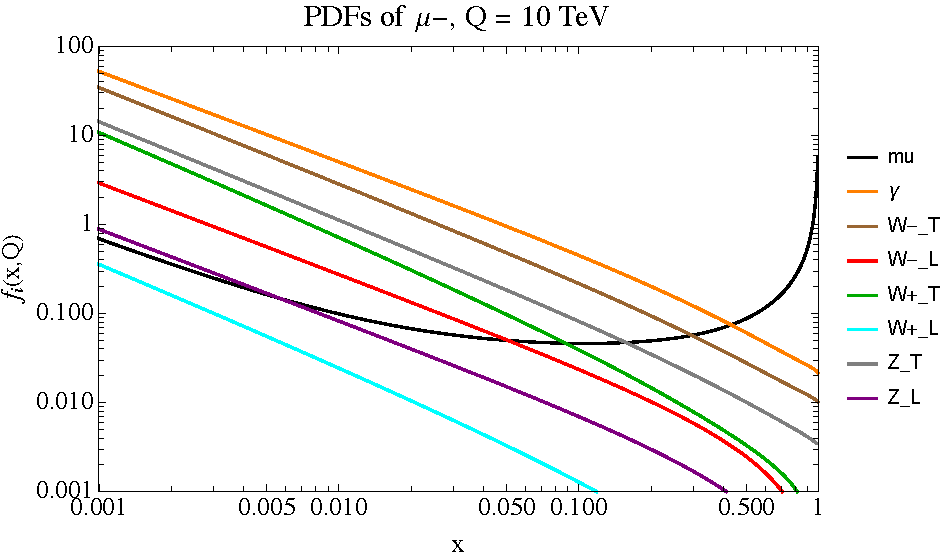
\includegraphics[width=0.46\linewidth]{Notebooks/PlotPDFs/alltogether/10TeV_mu-scaleQ.pdf}
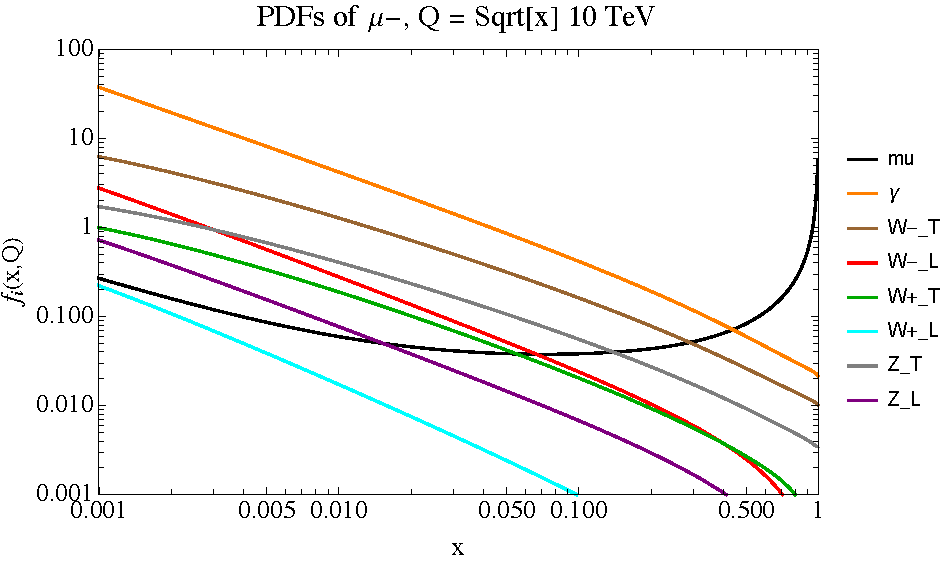
\includegraphics[width=0.46\linewidth]{Notebooks/PlotPDFs/alltogether/10TeV_mu-scaleQsqrtx.pdf}
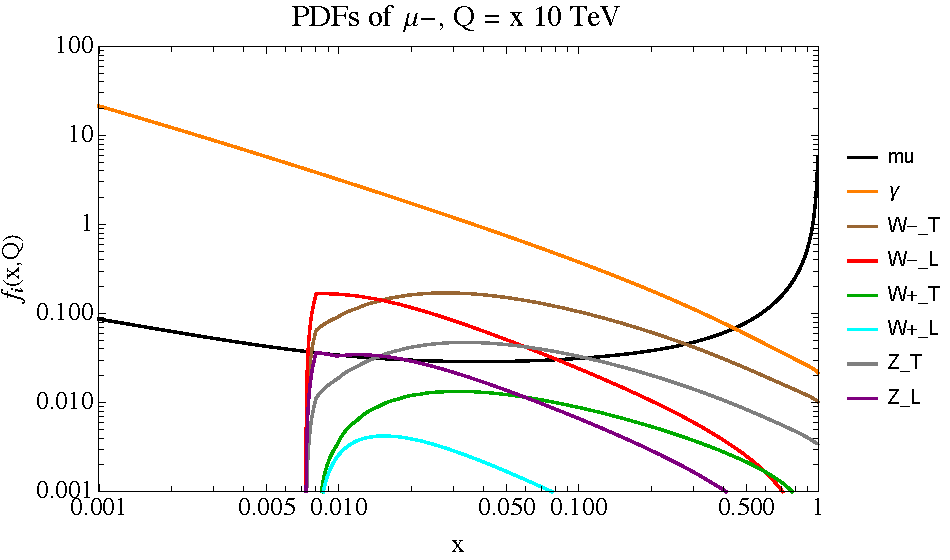
\includegraphics[width=0.46\linewidth]{Notebooks/PlotPDFs/alltogether/10TeV_mu-scaleQx.pdf}
\caption{PDF of the $\mu^-$ with different scale choices. \label{fig:allmum}}
\end{figure}


\begin{figure}[ht]
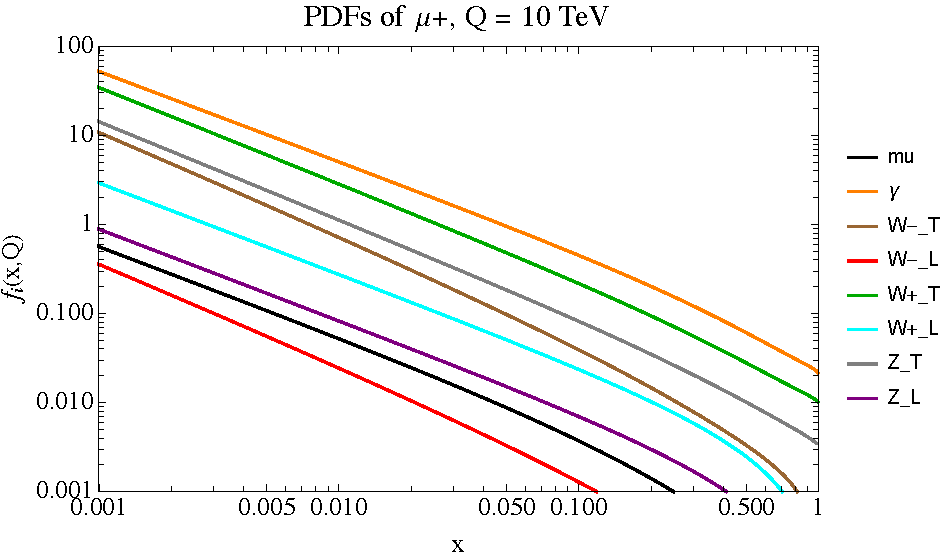
\includegraphics[width=0.46\linewidth]{Notebooks/PlotPDFs/alltogether/10TeV_mu+scaleQ.pdf}
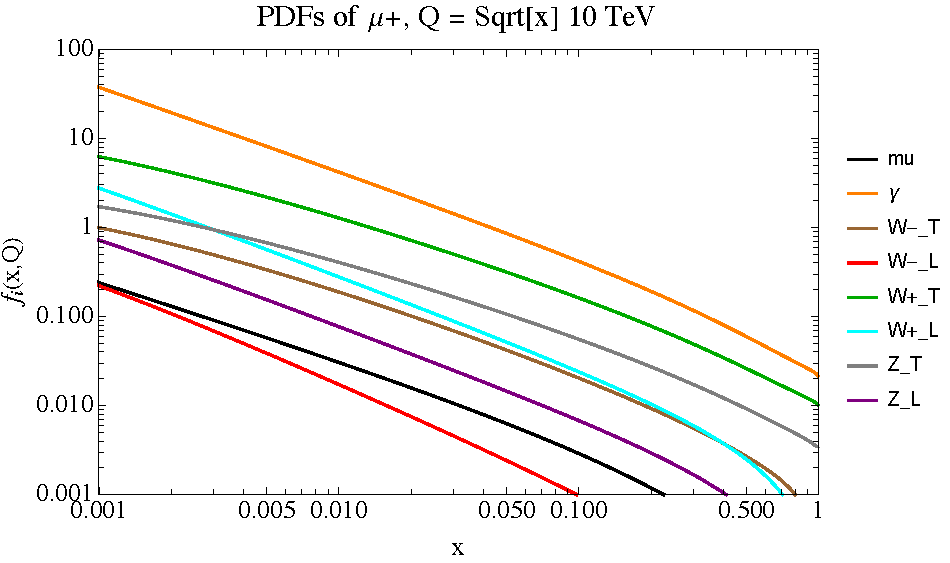
\includegraphics[width=0.46\linewidth]{Notebooks/PlotPDFs/alltogether/10TeV_mu+scaleQsqrtx.pdf}
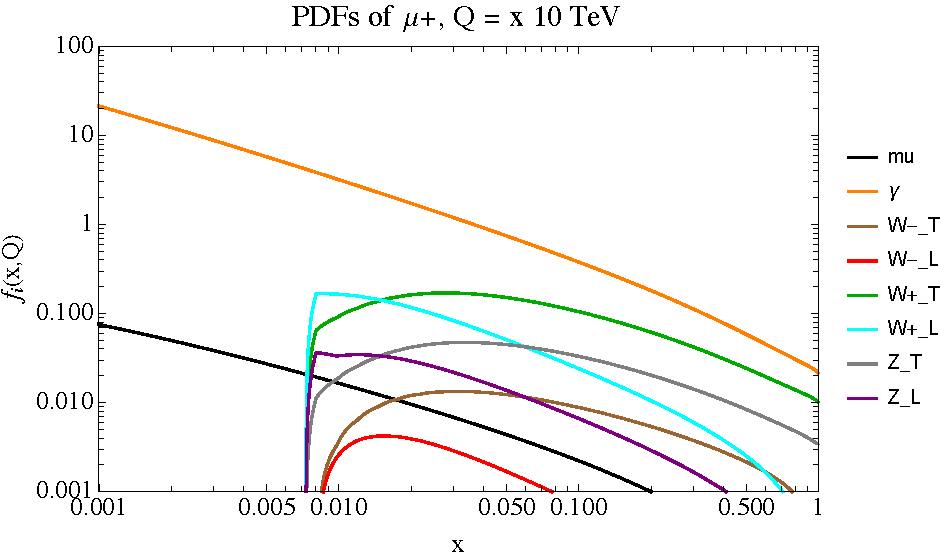
\includegraphics[width=0.46\linewidth]{Notebooks/PlotPDFs/alltogether/10TeV_mu+scaleQx.pdf}
\caption{PDF of the $\mu^{\color{red} +}$ with different scale choices, for the same partons. \label{fig:allmup}}
\end{figure}


We also show representative luminosities using the same PDFs, where the luminosity for producing a system of mass $M$ in a collider with squared energy $s$ (so $\tau=M^2/s$) is defined as

\begin{equation}
\mathcal L(M,s,Q)=\int_{M^2/s}^1 \frac{1}{x} f_1(x,Q) f_2(M^2/(x s),Q) dx\, ,
\end{equation}
where $Q$ is the factorisation scale chosen.

A physically motivated choice for $Q$ is precisely $M$ or a variation by a factor of 2 around it. In fact, as we will see later the case $M/2$ seems to better reproduce results from ME. Nevertheless, plugging Q=M in the definition before we recover the more common

\begin{equation}
\mathcal L(M,s,Q=M)=\int_{\tau}^1 \frac{1}{x} f_1(x,M) f_2(\tau/x,M) dx\, , \label{eq:lumicommon}
\end{equation}

The three choices of scale in Figs.~\ref{fig:allmum} and \ref{fig:allmup} correspond therefore to 

\begin{itemize}
\item $Q=\sqrt{s}$, which is not very well suited for the small-$x$ region where PDFs of $Z$ and $W$ are relevant. If $Q=M$ as in Eq.~\eqref{eq:lumicommon} this case is equivalent only for $x\to 1$.
\item$Q=\sqrt{x} \sqrt{s}$: If $Q=M$ as in Eq.~\eqref{eq:lumicommon} this case is equivalent in the region $x\to \sqrt{\tau}$. For luminosities as $WW$ or $ZZ$ this is the best case to look at, in my opinion. Take $M$ and $S$, look at $\sqrt{\tau}$ and one can have a comparison for the bulk of the contribution of the different PDFs
\item $Q=x \sqrt{s}$: If $Q=M$ as in Eq.~\eqref{eq:lumicommon} this case is equivalent in the region $x \to \tau$. It is the opposite of the region $x\to 1$ and indeed, for $M=\mw$, where EW PDFs collapses, $\tau \simeq 0.008$, which we see in the plot.    
\end{itemize}


In Fig.~\ref{fig:lumicomparison} we show the comparison of representative luminosities with {\small \sc LePDF}, with the scale set at $Q=M/2$.
Comparisons for same luminosities with different polarisation are shown in the corresponding section later.


%NIntegrate[ 1/x \[Mu]EVApartv2[part1, m\[Mu]\[Mu]*muoverm\[Mu]\[Mu], 
%   x] \[Mu]bEVApartv2[part2, m\[Mu]\[Mu]*muoverm\[Mu]\[Mu], 
%   m\[Mu]\[Mu]^2/(x sqrts0^2)], {x, m\[Mu]\[Mu]^2/sqrts0^2, 1}  

\begin{figure}
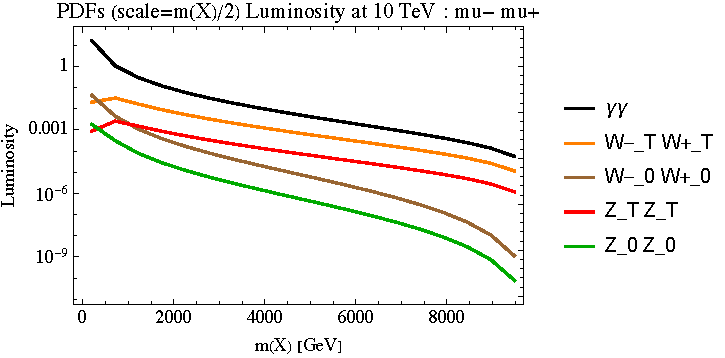
\includegraphics[width=0.9\linewidth]{Notebooks/PlotLumi/10TeV/lumis/plotgammaWZ.pdf} 
\caption{Comparison of luminosities \label{fig:lumicomparison}}
\end{figure}

 
\clearpage

\section{$ZZ$ initiated $t \bar t$ production}

We start analysing the $ZZ\to t \bar t$ process, which is a VBF subcomponent of the complete process (ME) $\mu^+\mu^-\to\mu^+\mu^- t \bar t$. As it is clear, this process involves also the VBF process $\gamma \gamma \to t \bar t$, which is dominant. This can be guessed from Fig.~\ref{fig:lumicomparison} and by the fact that $\log(m(t\bar t)/m_\mu)\gg \log(m(t\bar t)/m_Z)$. Moreover, this process features also a $\mu^+\mu^-\to- t \bar t \gamma (\gamma\to t \bar t )$ topology, which in a massless computation would be removed at NNLO. \footnote{Still, we have verified this contribution to be negligible w.r.t.~our NNLO total phenomenological prediction when a cut on $m(\mu^+ \mu-)$ is applied }Luckily, for such process the purely QED and purely weak component of the $\mu^+\mu^-\to\mu^+\mu^- t \bar t$ amplitude can be separated in a gauge invariant way, therefore we veto the photons in the amplitude. In order to be as close as possible to the $VBF$ configuration we avoid also the process $\mu^+\mu^-\to- t \bar t Z (Z \to t \bar t )$, by actually generating the ME as $\mu^+e^-\to\mu^+e^- t \bar t$ and setting the mass and the Yukawa of the electron equal to the one of the muon. We denote in the plots such prediction as ME no-QED.

We start with a set of cuts defined as follows
%
\begin{equation}
m(t \bar t) > 500~\gev, p_T(t/ \bar t) > 150~\gev, |\eta(t/\bar t)|<2.5 
\end{equation}
%
we show in Fig.~\ref{fig:cutsZZtt} the $m(t \bar t)$ distribution at ME-noQED versus the EVA predictions using the notation of Ref.~\cite{Garosi:2023bvq} with a central scale definition for the EVA $\mu=m(t \bar t) /2$ and a variation around it by a factor of 2.
We also explicitly  show the ratio of the EVA predictions with the ME-noQED one. The same plot is also shown for parameterisation of the EVA from Ref.~\cite{Ruiz:2021tdt}, which we denoted in the plots as ``EVA only Log[mu/MV]''.

For both EVA definitions we observe a good agreement within the scale uncertainty band with the EVA-noQED. The case $\mu=m(t \bar t)/2$ is actually at the a few percents from the  EVA-noQED, and at 10\% for the case  ``EVA only Log[mu/MV]''. Still the scale uncertainty band is at the $\pm40\%$ level.

This good agreement deteriorates if the $\eta(t)$ distribution is considered. \pnote{I fear there is a bug here, and EVA results could be in the partonic res frame. The same applies in all the other eta plots. The bug is not present for the invariant mass because it is Lrentz-invariant. To be checked!} 

 


\begin{figure}[ht]
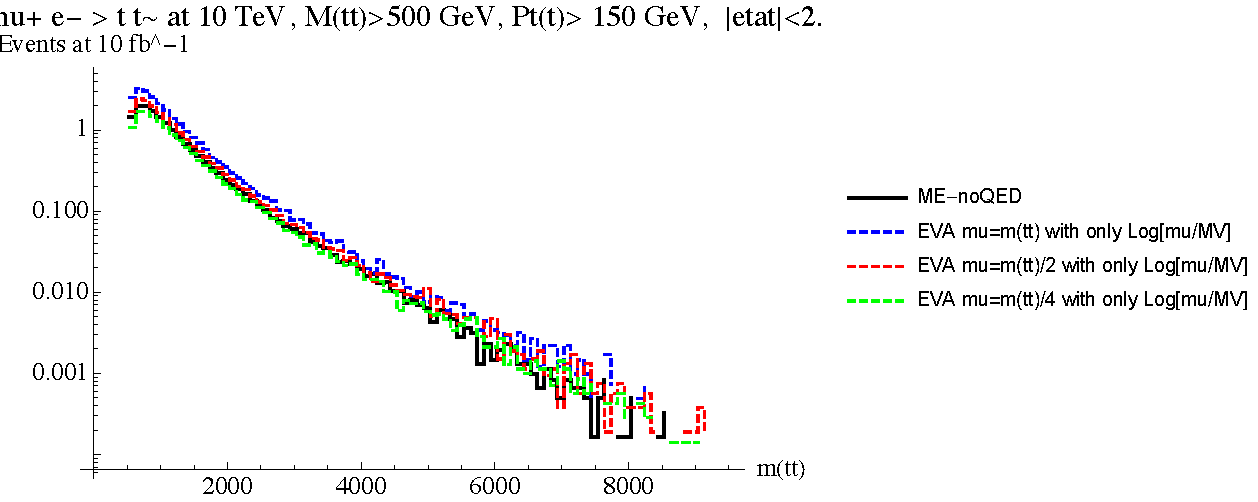
\includegraphics[width=0.46\linewidth]{Notebooks/PlotDistr/ZZ_tt/10TeVcuts/plotmtt.pdf}
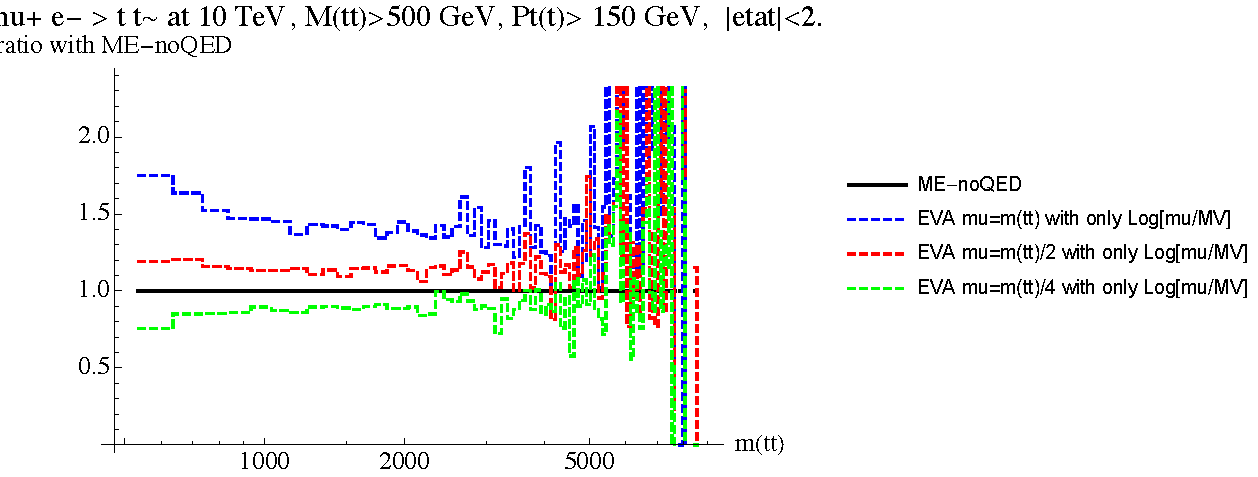
\includegraphics[width=0.46\linewidth]{Notebooks/PlotDistr/ZZ_tt/10TeVcuts/plotmttratio1.pdf}
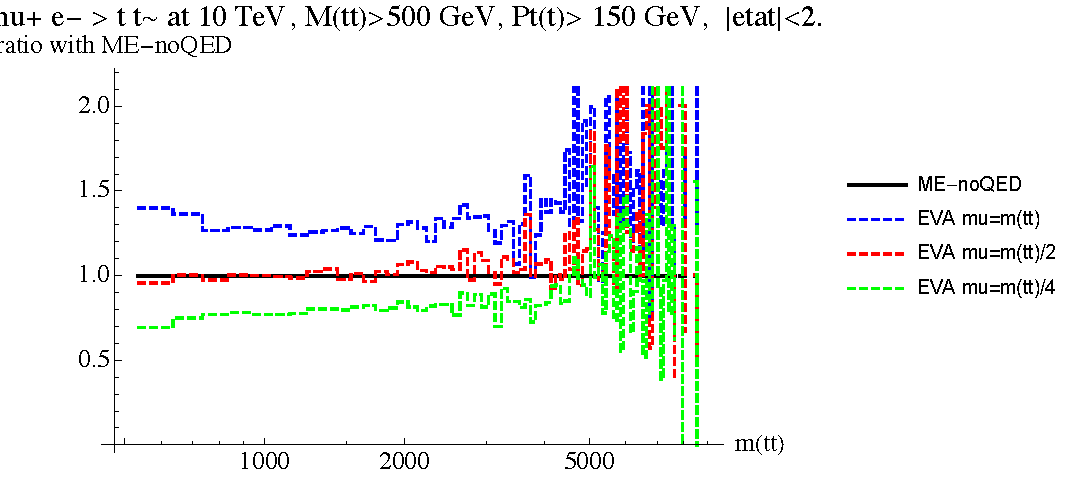
\includegraphics[width=0.46\linewidth]{Notebooks/PlotDistr/ZZ_tt/10TeVcuts/plotmttratio2.pdf}
\label{fig:cutsZZtt}
\end{figure}


\begin{figure}[ht]
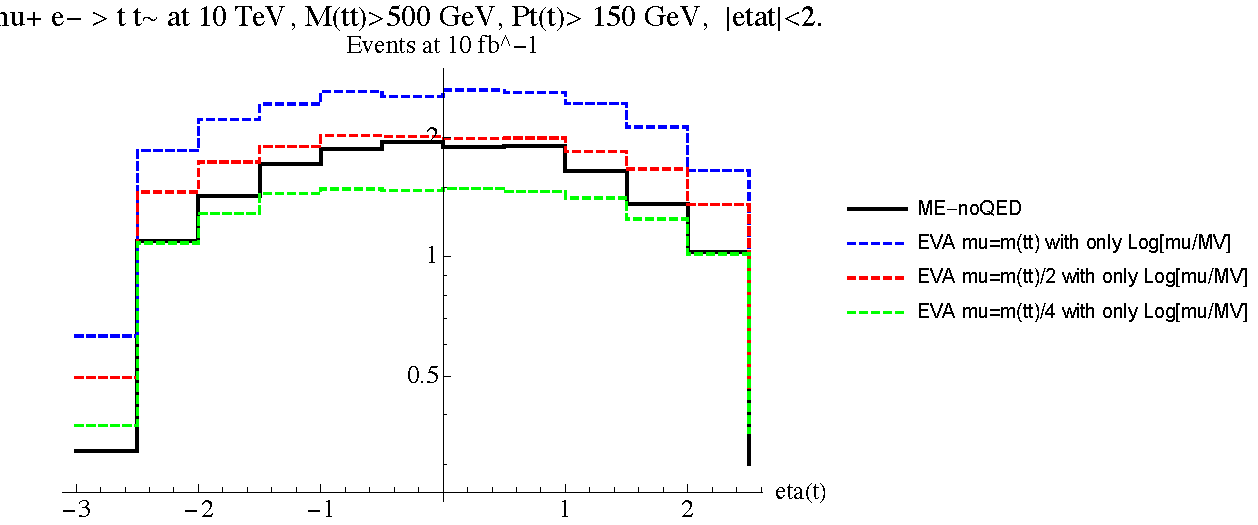
\includegraphics[width=0.46\linewidth]{Notebooks/PlotDistr/ZZ_tt/10TeVcuts/plotetat.pdf}
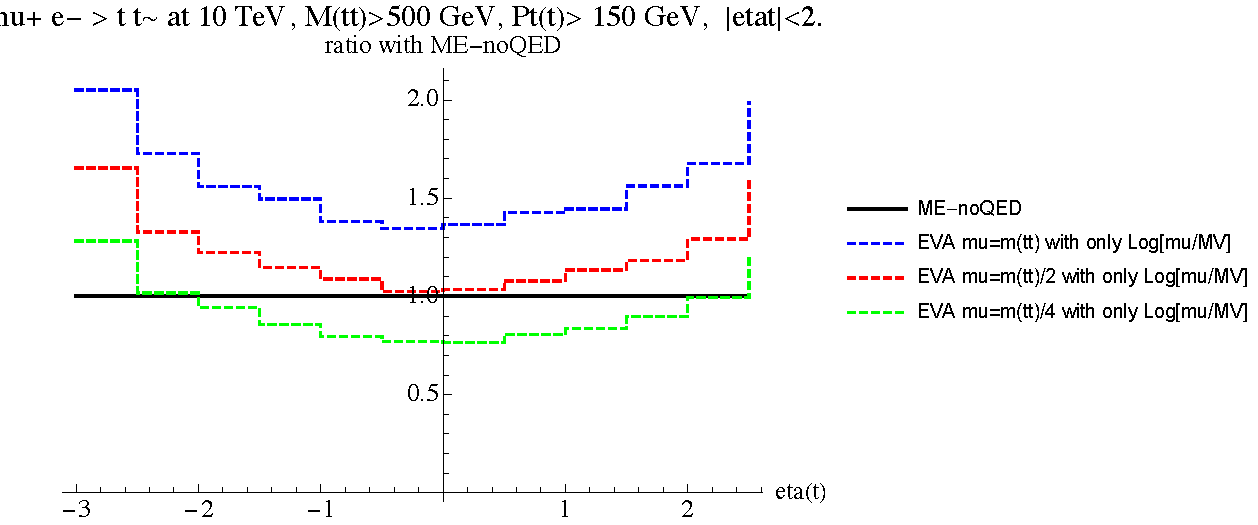
\includegraphics[width=0.46\linewidth]{Notebooks/PlotDistr/ZZ_tt/10TeVcuts/plotetatratio1.pdf}
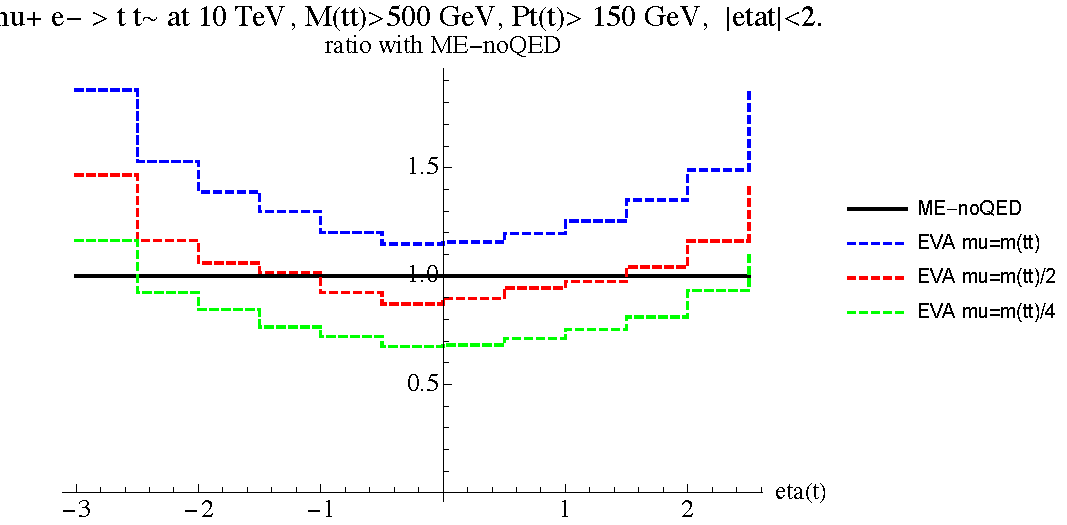
\includegraphics[width=0.46\linewidth]{Notebooks/PlotDistr/ZZ_tt/10TeVcuts/plotetatratio2.pdf}
\end{figure}


\begin{figure}[ht]
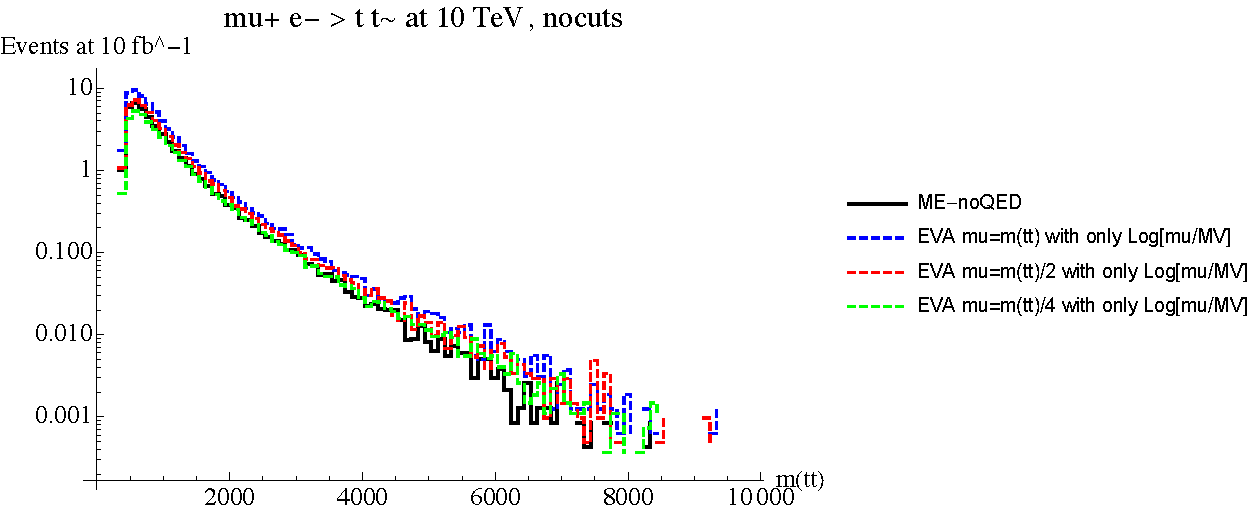
\includegraphics[width=0.46\linewidth]{Notebooks/PlotDistr/ZZ_tt/10TeVnocuts/plotmtt.pdf}
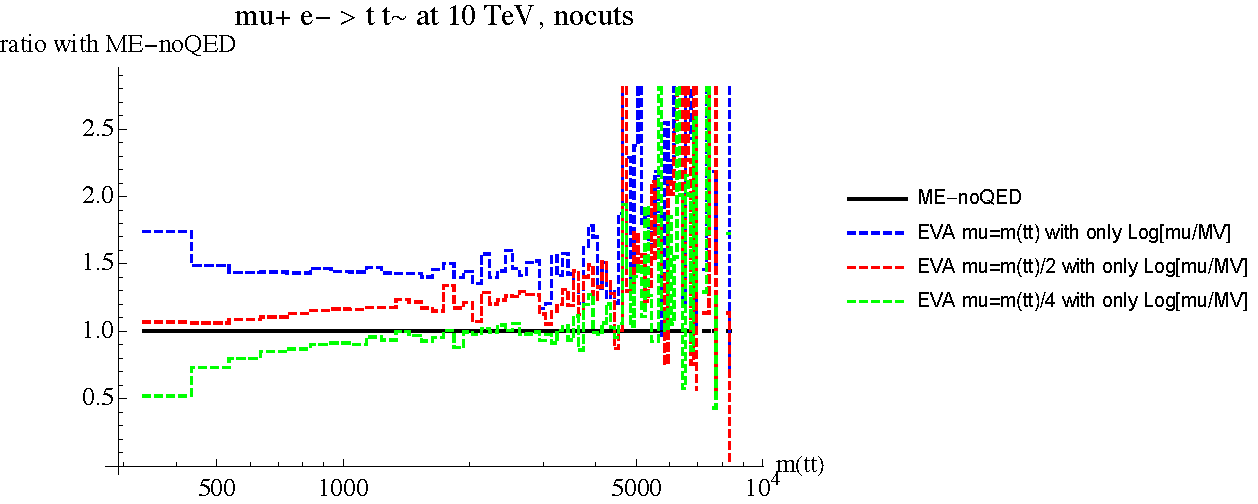
\includegraphics[width=0.46\linewidth]{Notebooks/PlotDistr/ZZ_tt/10TeVnocuts/plotmttratio1.pdf}
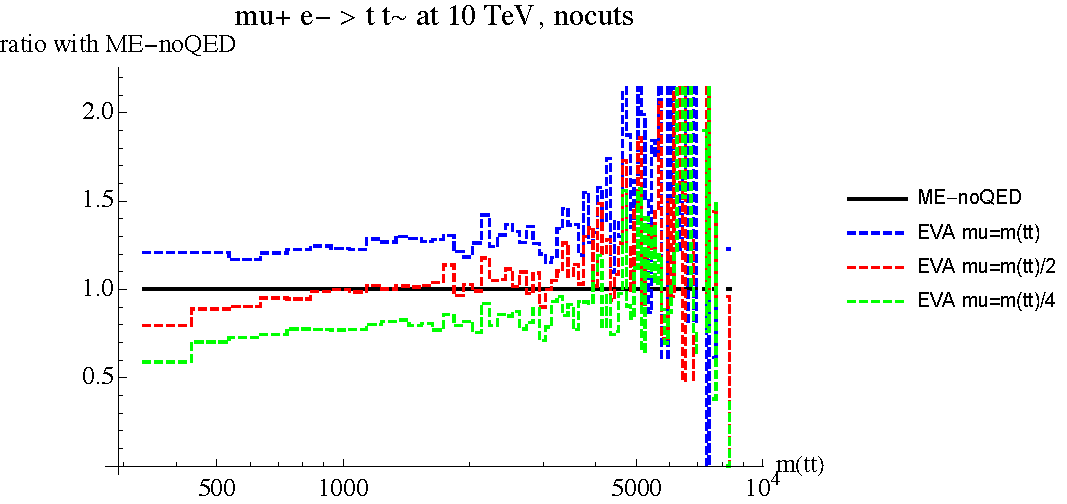
\includegraphics[width=0.46\linewidth]{Notebooks/PlotDistr/ZZ_tt/10TeVnocuts/plotmttratio2.pdf}
\end{figure}


\begin{figure}[ht]
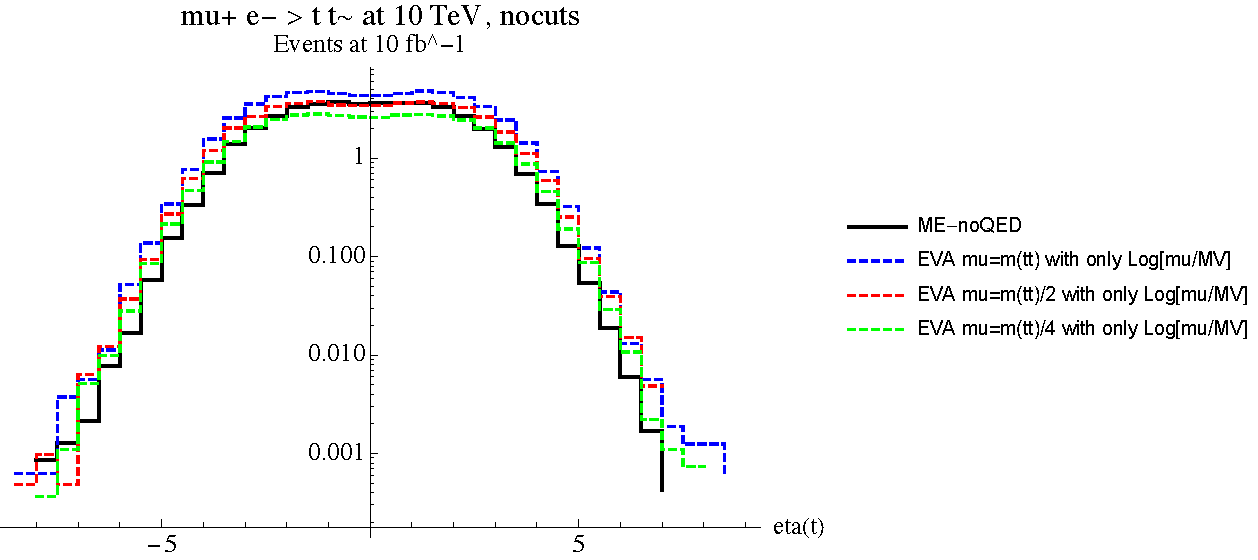
\includegraphics[width=0.46\linewidth]{Notebooks/PlotDistr/ZZ_tt/10TeVnocuts/plotetat.pdf}
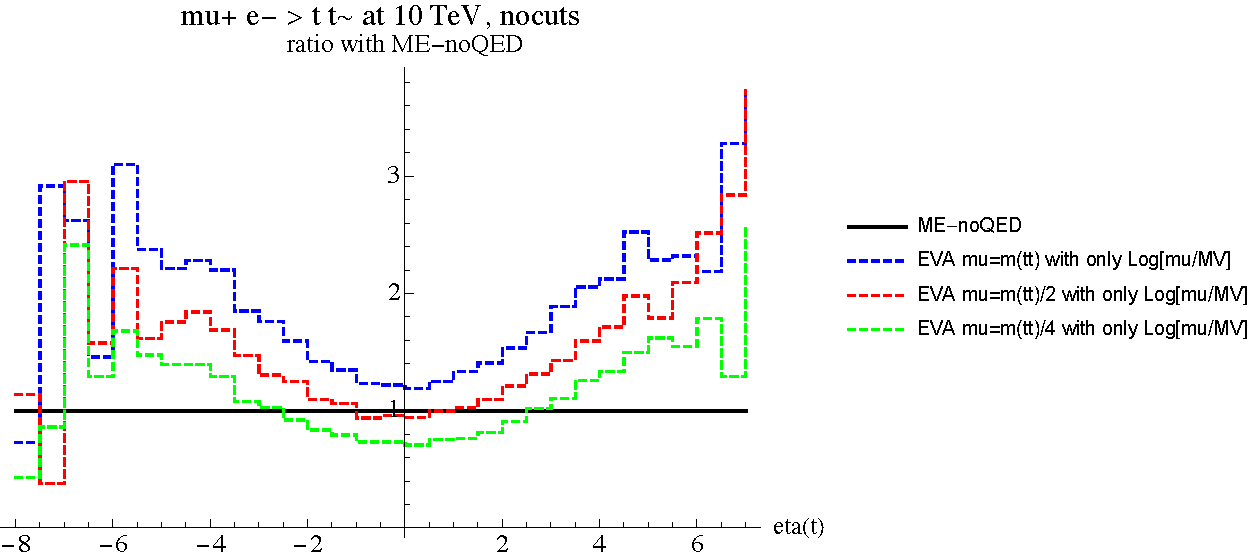
\includegraphics[width=0.46\linewidth]{Notebooks/PlotDistr/ZZ_tt/10TeVnocuts/plotetatratio1.pdf}
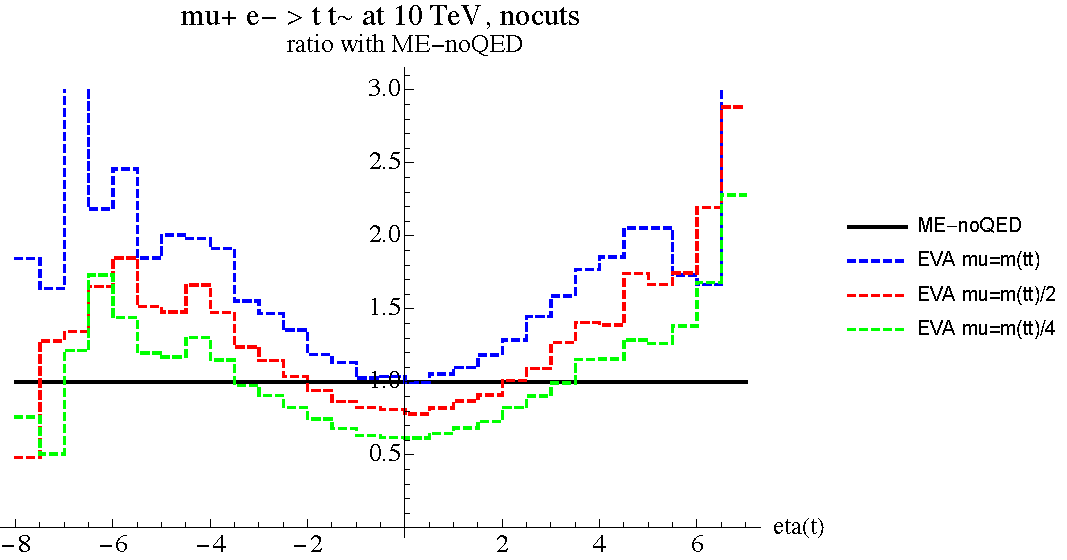
\includegraphics[width=0.46\linewidth]{Notebooks/PlotDistr/ZZ_tt/10TeVnocuts/plotetatratio2.pdf}
\end{figure}




%\begin{figure}[ht]
%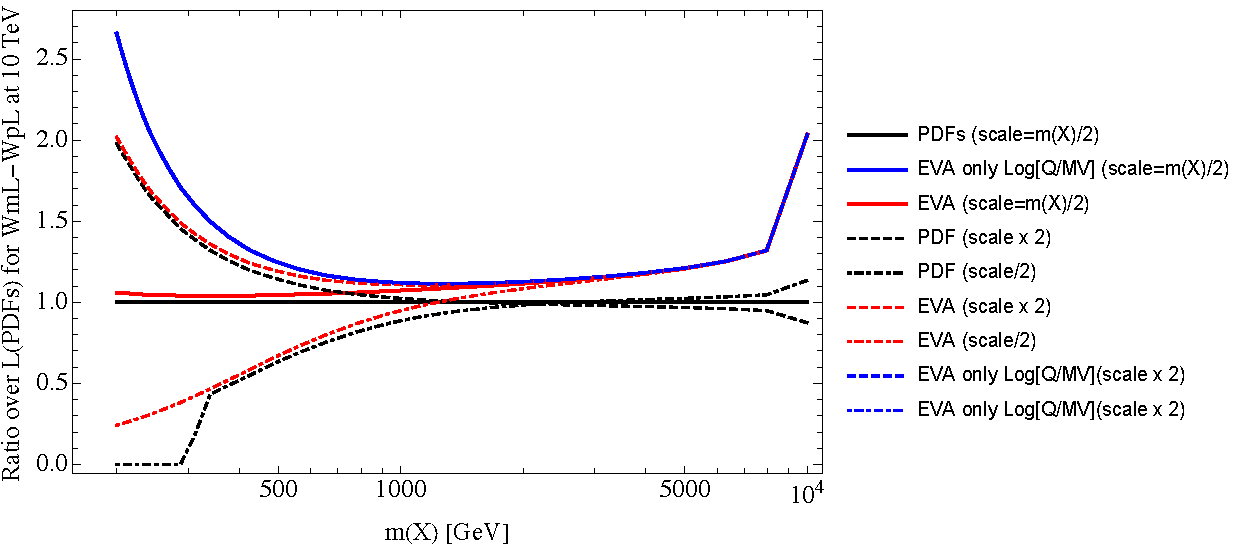
\includegraphics[width=0.46\linewidth]{Notebooks/PlotLumi/10TeV/ratios/WmL-WpL.pdf}
%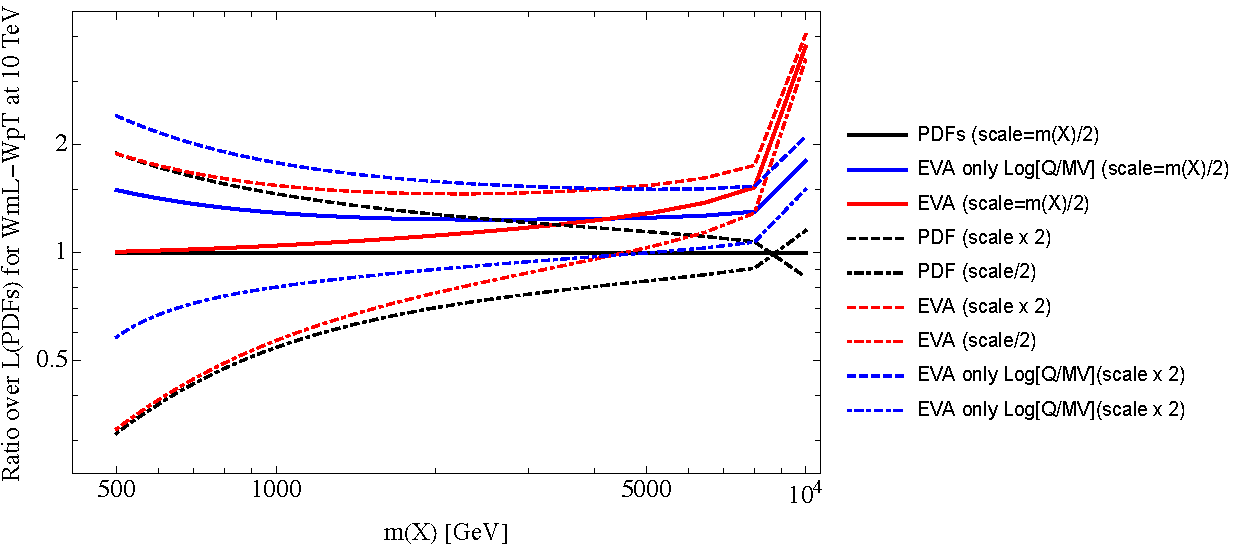
\includegraphics[width=0.46\linewidth]{Notebooks/PlotLumi/10TeV/ratios/WmL-WpT.pdf}
%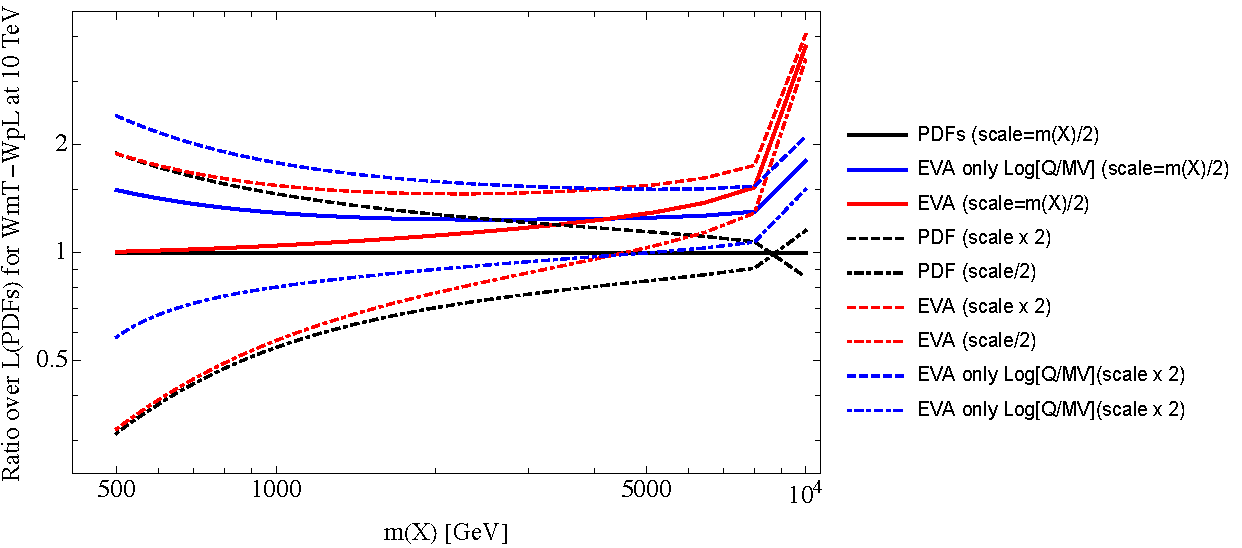
\includegraphics[width=0.46\linewidth]{Notebooks/PlotLumi/10TeV/ratios/WmT-WpL.pdf}
%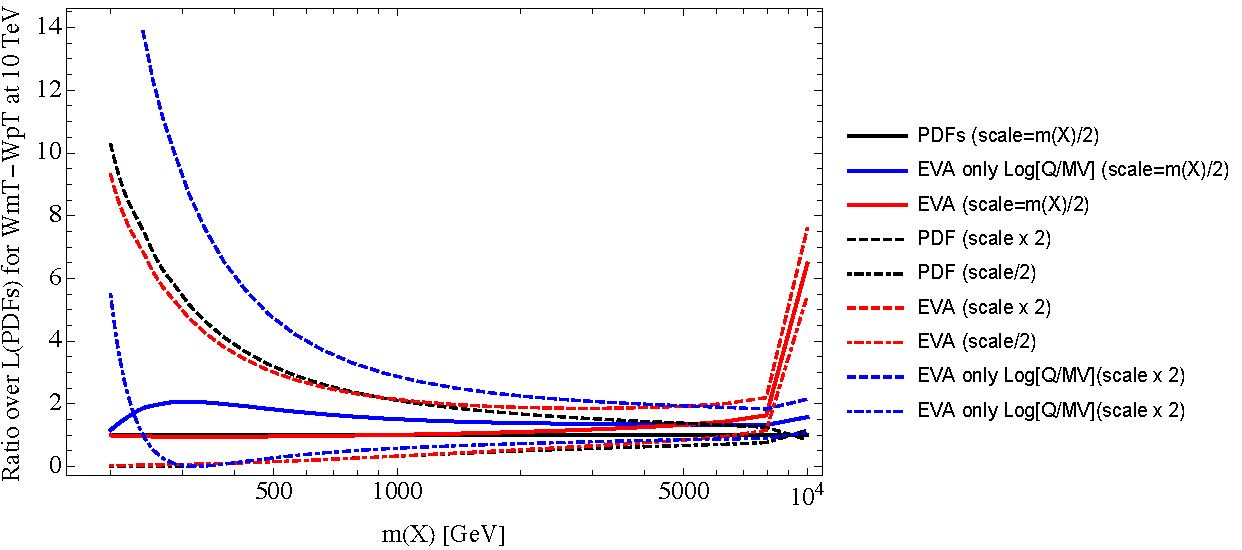
\includegraphics[width=0.46\linewidth]{Notebooks/PlotLumi/10TeV/ratios/WmT-WpT.pdf}
%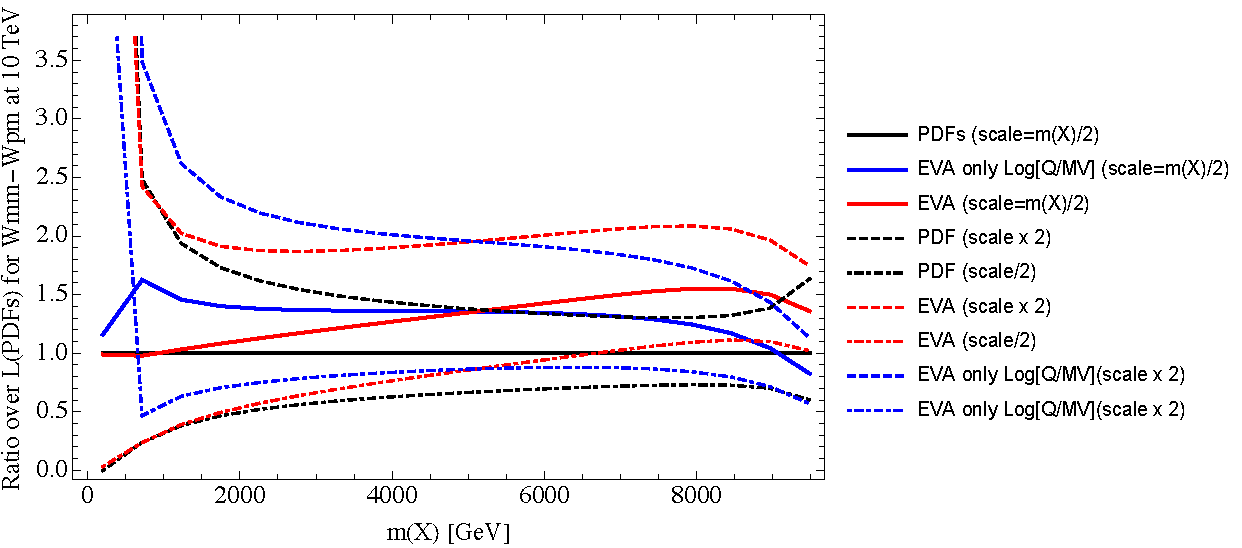
\includegraphics[width=0.46\linewidth]{Notebooks/PlotLumi/10TeV/ratios/Wmm-Wpm.pdf}
%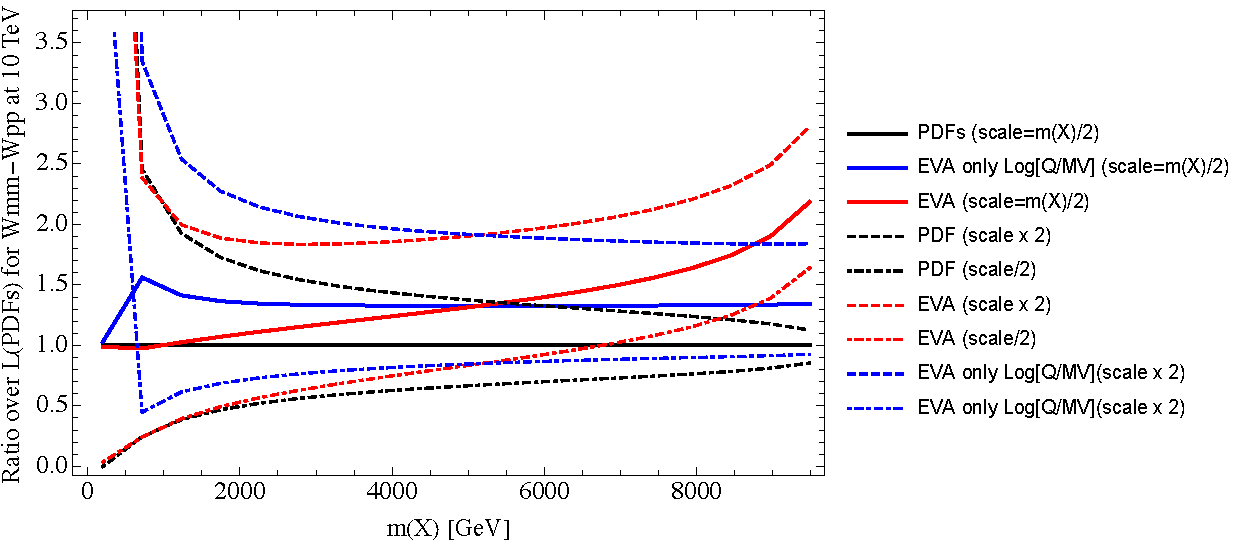
\includegraphics[width=0.46\linewidth]{Notebooks/PlotLumi/10TeV/ratios/Wmm-Wpp.pdf}
%\end{figure}
%
%\begin{figure}[ht]
%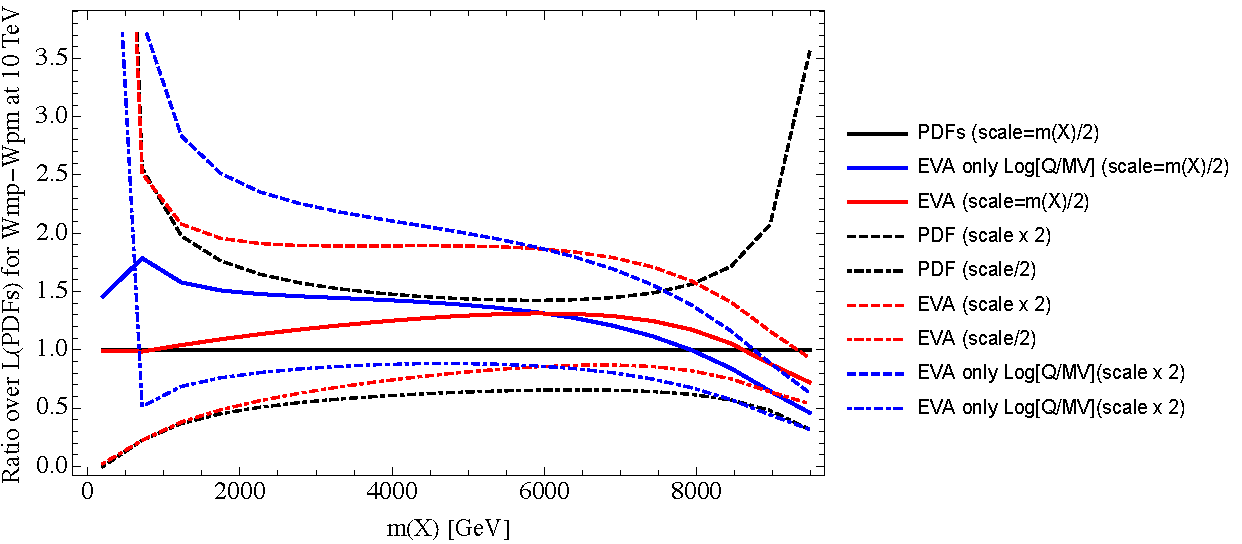
\includegraphics[width=0.46\linewidth]{Notebooks/PlotLumi/10TeV/ratios/Wmp-Wpm.pdf}
%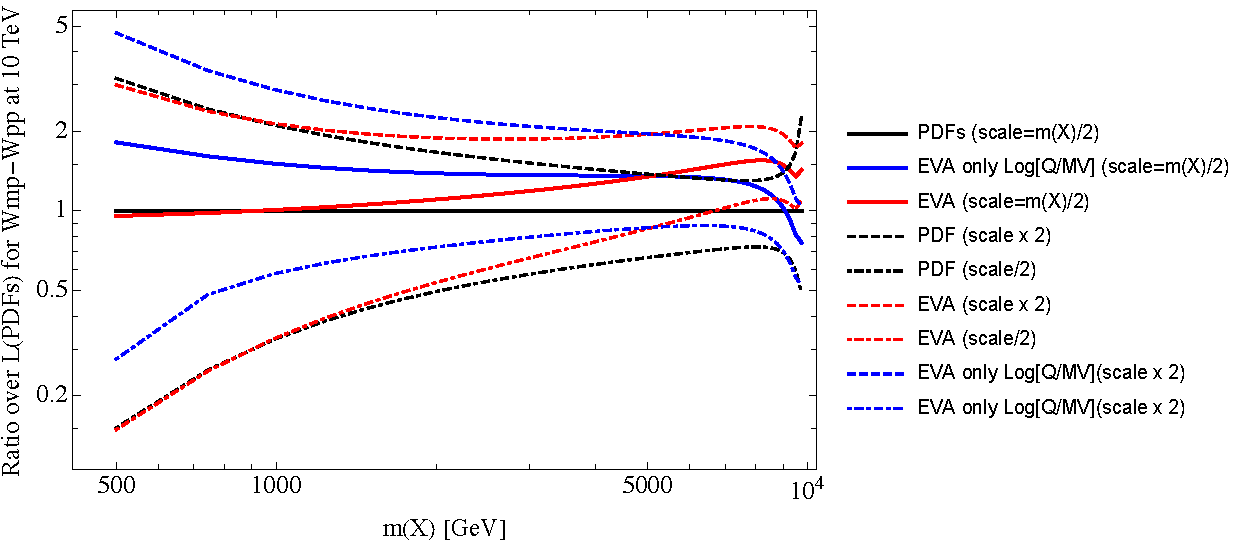
\includegraphics[width=0.46\linewidth]{Notebooks/PlotLumi/10TeV/ratios/Wmp-Wpp.pdf}

\begin{figure}[ht]
%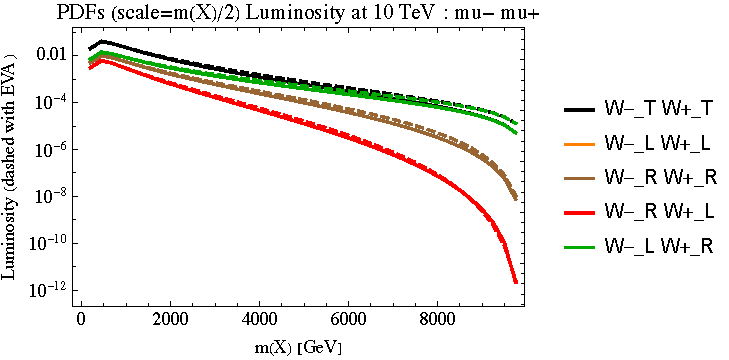
\includegraphics[width=0.46\linewidth]{Notebooks/PlotLumi/10TeV/lumis/plotWWpolRandL.pdf}
%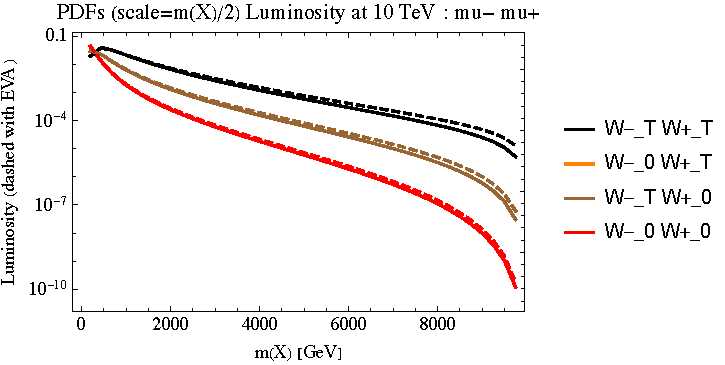
\includegraphics[width=0.46\linewidth]{Notebooks/PlotLumi/10TeV/lumis/plotWWpolTand0.pdf}
%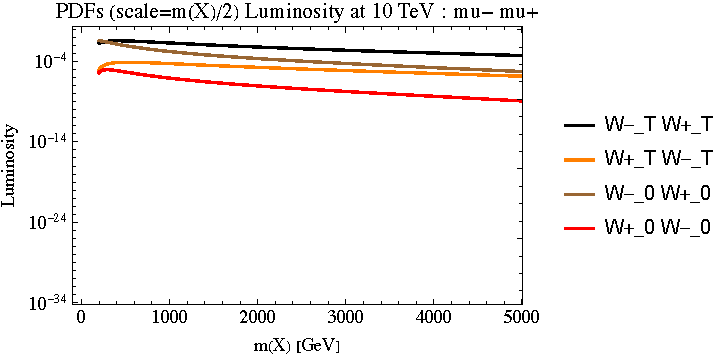
\includegraphics[width=0.46\linewidth]{Notebooks/PlotLumi/10TeV/lumis/plotWmWpandWpWm.pdf}
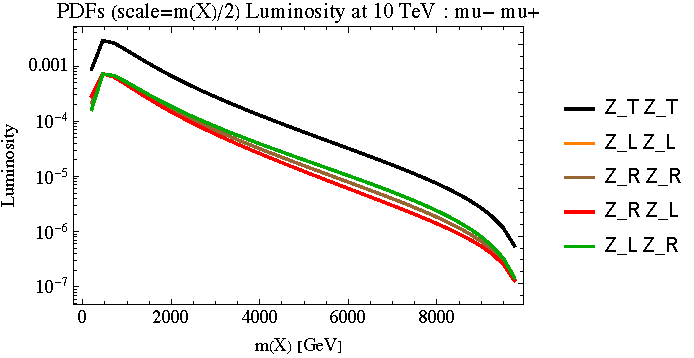
\includegraphics[width=0.46\linewidth]{Notebooks/PlotLumi/10TeV/lumis/plotZZpolRandL.pdf}
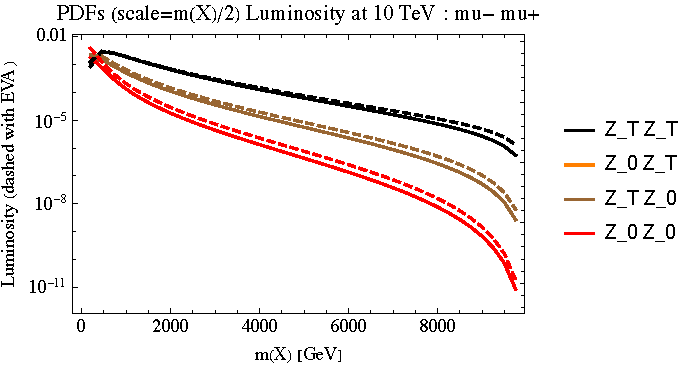
\includegraphics[width=0.46\linewidth]{Notebooks/PlotLumi/10TeV/lumis/plotZZpolTand0.pdf}
\end{figure}





\begin{figure}[ht]
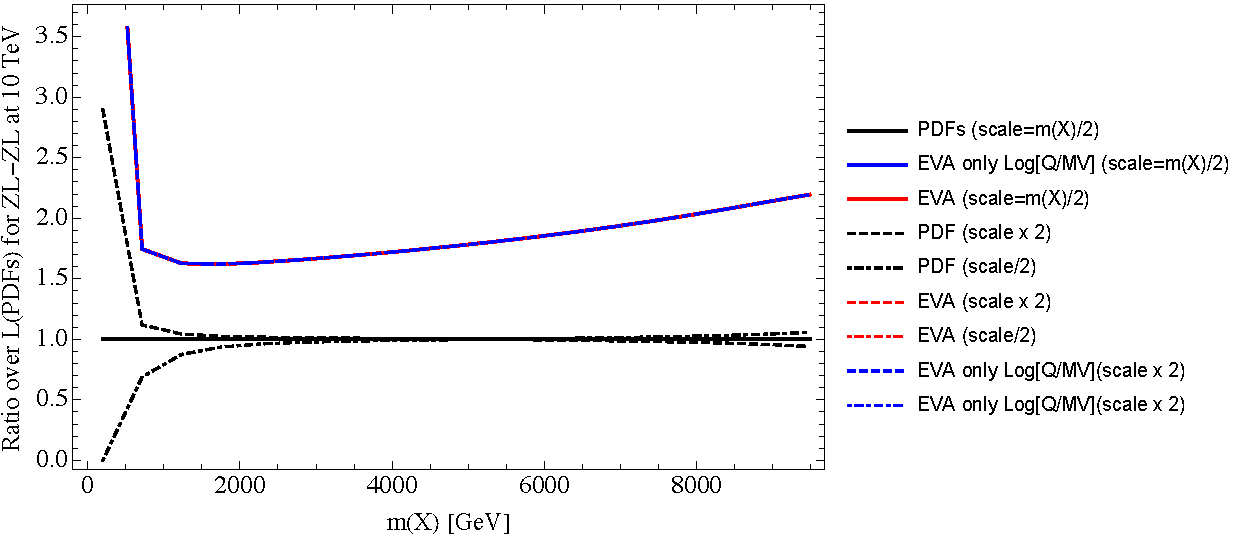
\includegraphics[width=0.46\linewidth]{Notebooks/PlotLumi/10TeV/ratios/ZL-ZL.pdf}
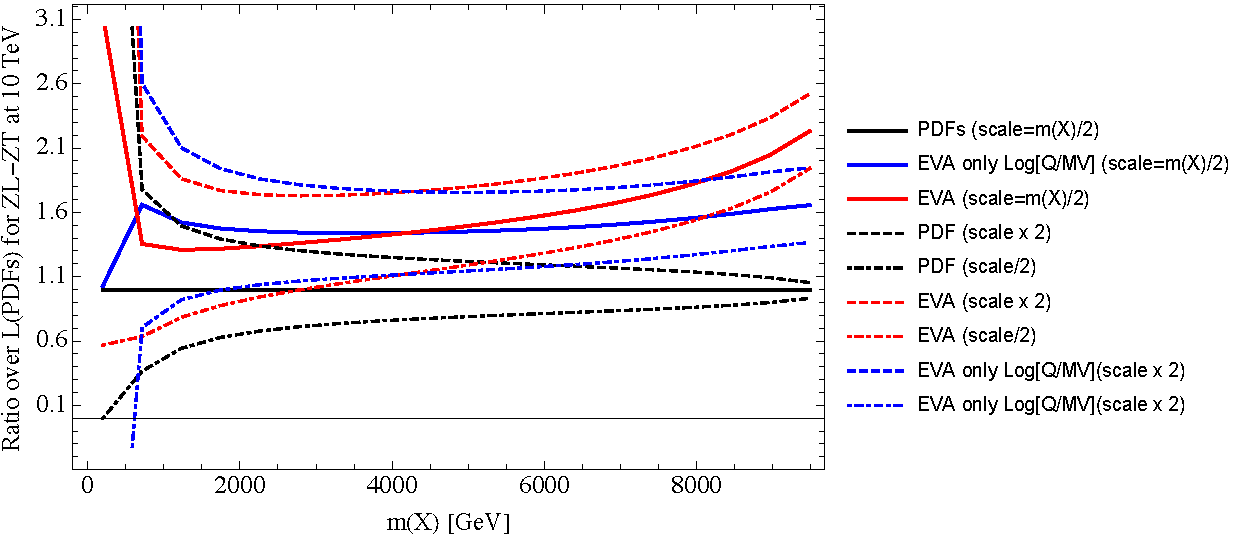
\includegraphics[width=0.46\linewidth]{Notebooks/PlotLumi/10TeV/ratios/ZL-ZT.pdf}
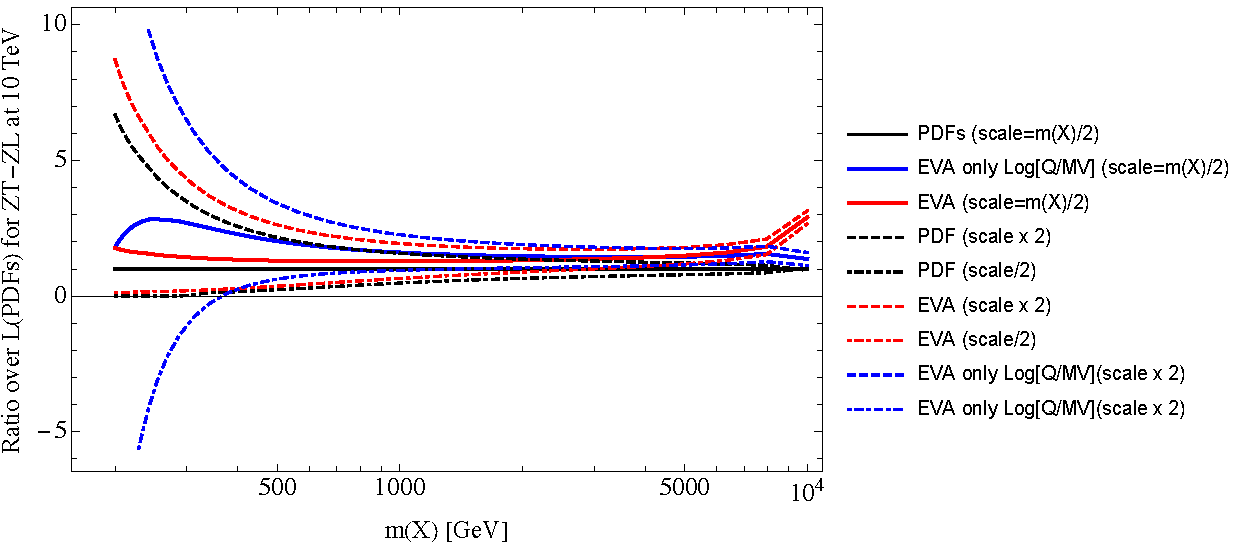
\includegraphics[width=0.46\linewidth]{Notebooks/PlotLumi/10TeV/ratios/ZT-ZL.pdf}
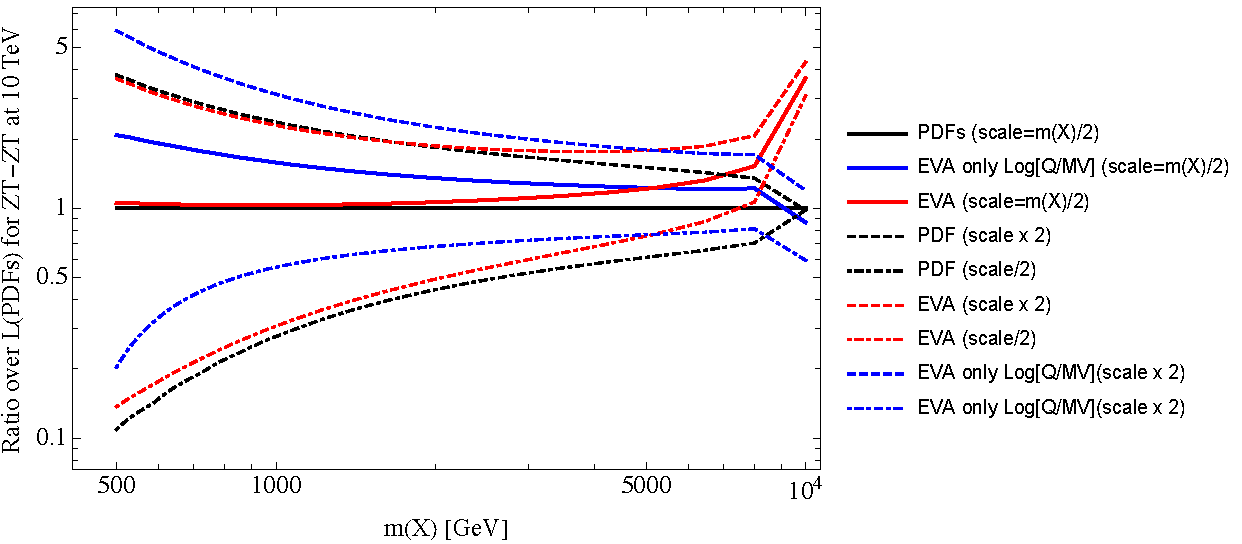
\includegraphics[width=0.46\linewidth]{Notebooks/PlotLumi/10TeV/ratios/ZT-ZT.pdf}
\end{figure}

\begin{figure}[ht]
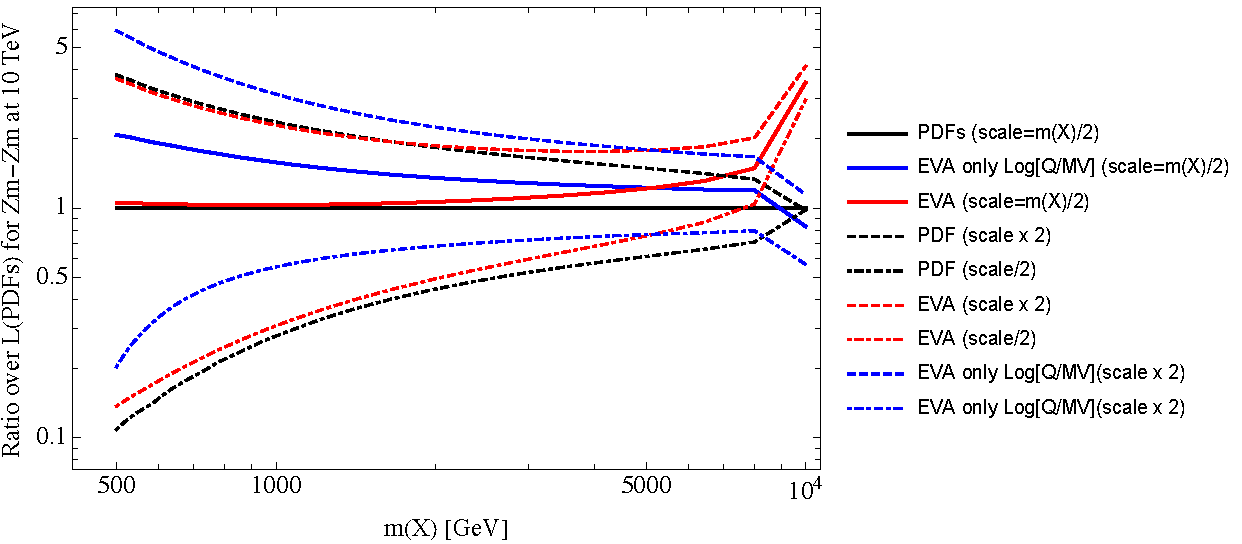
\includegraphics[width=0.46\linewidth]{Notebooks/PlotLumi/10TeV/ratios/Zm-Zm.pdf}
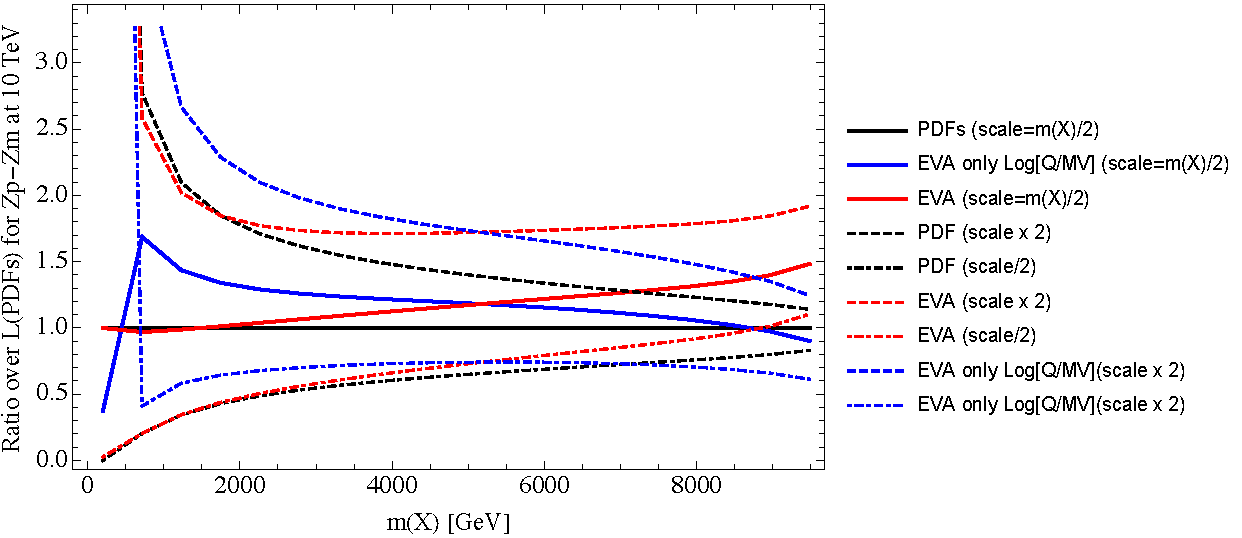
\includegraphics[width=0.46\linewidth]{Notebooks/PlotLumi/10TeV/ratios/Zp-Zm.pdf}
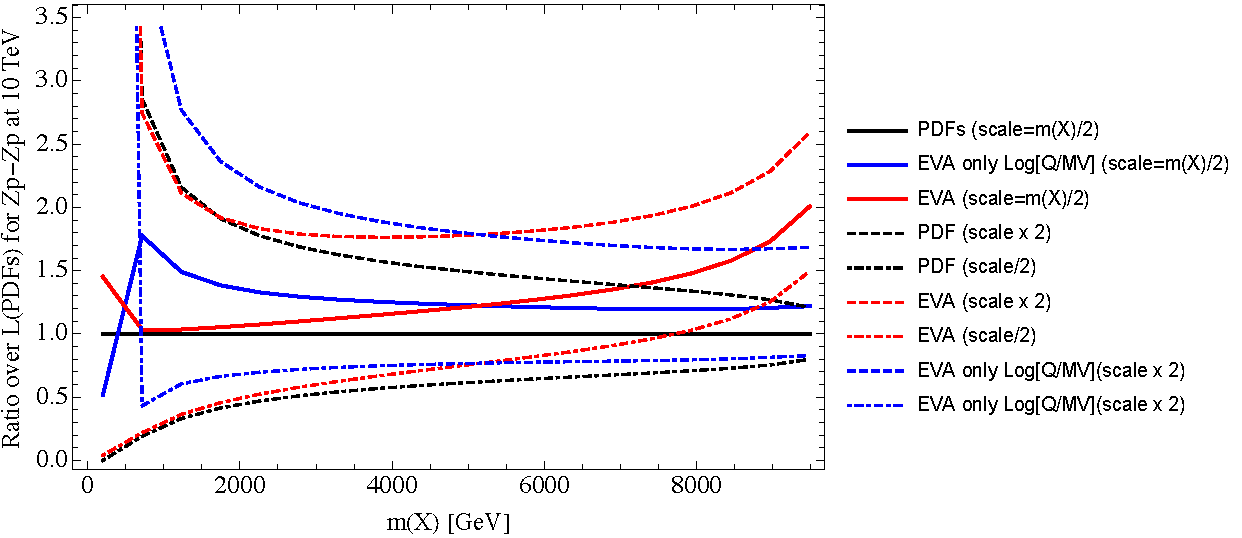
\includegraphics[width=0.46\linewidth]{Notebooks/PlotLumi/10TeV/ratios/Zp-Zp.pdf}
\end{figure}




\clearpage

%%%%%%%%%%%%%%%%%%%%%%%%%%%%%%%%%%%%%%
%%%%%%%%%%%%%%%%%%%%%%%%%%%%%%%%%%%%%%
%%%%%%%%%%%%%%%%%%%%%%%%%%%%%%%%%%%%%%
%%%%%%%%%%%%%%%%%%%%%%%%%%%%%%%%%%%%%%
%%%%%%%%%%%%%%%%%%%%%%%%%%%%%%%%%%%%%%
%%%%%%%%%%%%%%%%%%%%%%%%%%%%%%%%%%%%%%
%%%%%%%%%%%%%%%%%%%%%%%%%%%%%%%%%%%%%%
%%%%%%%%%%%%%%%%%%%%%%%%%%%%%%%%%%%%%%
%%%%%%%%%%%%%%%%%%%%%%%%%%%%%%%%%%%%%%
%%%%%%%%%%%%%%%%%%%%%%%%%%%%%%%%%%%%%%
%%%%%%%%%%%%%%%%%%%%%%%%%%%%%%%%%%%%%%
%%%%%%%%%%%%%%%%%%%%%%%%%%%%%%%%%%%%%%
%%%%%%%%%%%%%%%%%%%%%%%%%%%%%%%%%%%%%%
%%%%%%%%%%%%%%%%%%%%%%%%%%%%%%%%%%%%%%
%%%%%%%%%%%%%%%%%%%%%%%%%%%%%%%%%%%%%%
%%%%%%%%%%%%%%%%%%%%%%%%%%%%%%%%%%%%%%
%%%%%%%%%%%%%%%%%%%%%%%%%%%%%%%%%%%%%%
%%%%%%%%%%%%%%%%%%%%%%%%%%%%%%%%%%%%%%
%%%%%%%%%%%%%%%%%%%%%%%%%%%%%%%%%%%%%%
%%%%%%%%%%%%%%%%%%%%%%%%%%%%%%%%%%%%%%
%%%%%%%%%%%%%%%%%%%%%%%%%%%%%%%%%%%%%%
%%%%%%%%%%%%%%%%%%%%%%%%%%%%%%%%%%%%%%
%%%%%%%%%%%%%%%%%%%%%%%%%%%%%%%%%%%%%%





\appendix

\section{ME vs EVA}

\subsection{$WW$ into $WW$}


%\begin{figure}[ht]
%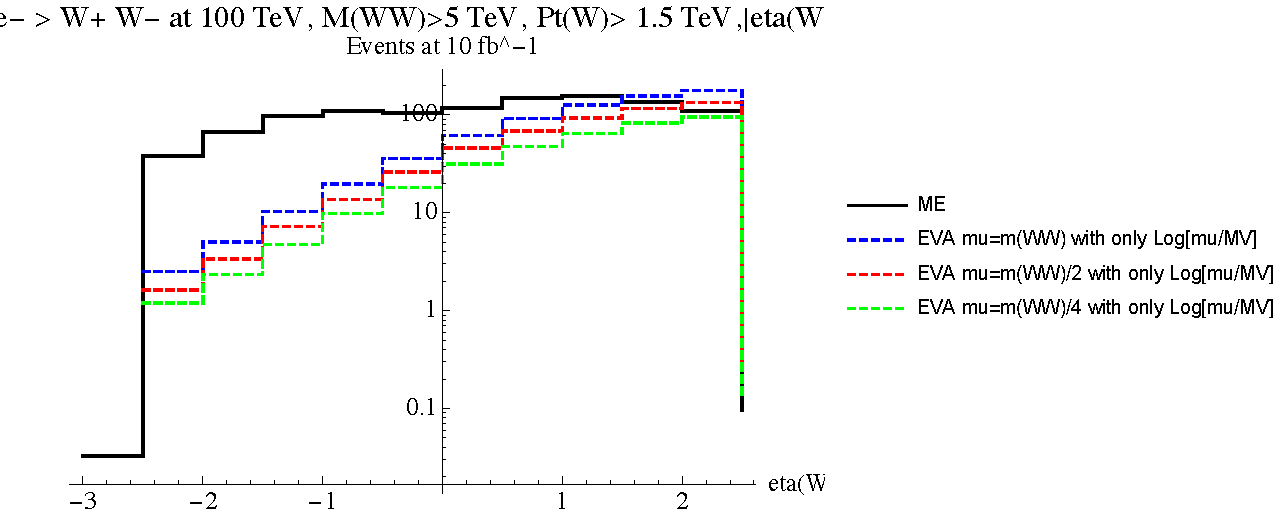
\includegraphics[width=0.46\linewidth]{Notebooks/PlotDistr/WW_WW/100TeVcuts/plotetaW.pdf}
%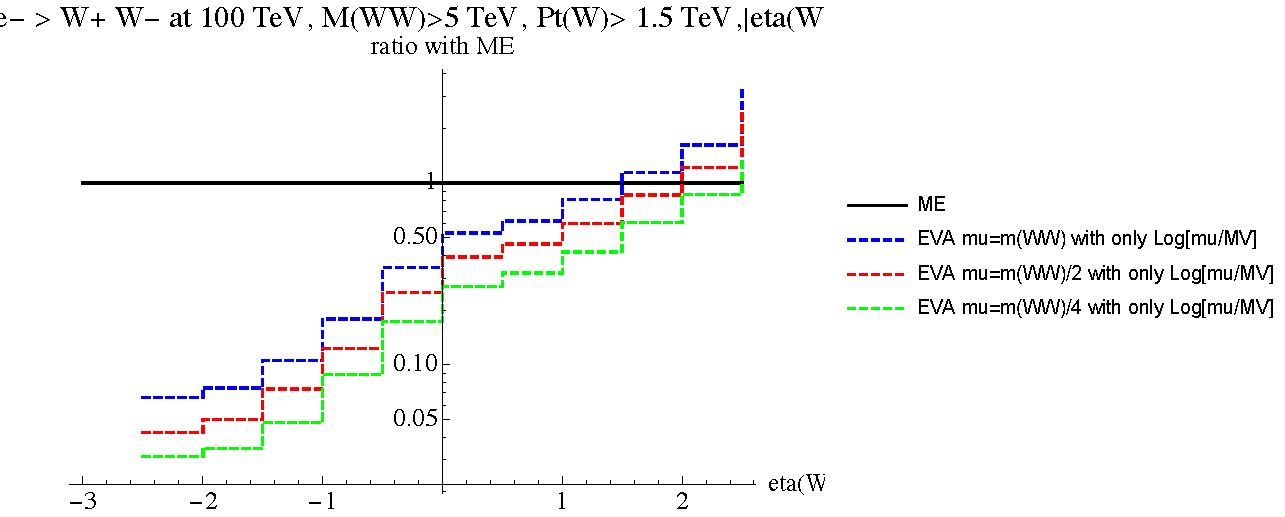
\includegraphics[width=0.46\linewidth]{Notebooks/PlotDistr/WW_WW/100TeVcuts/plotetaWratio1.pdf}
%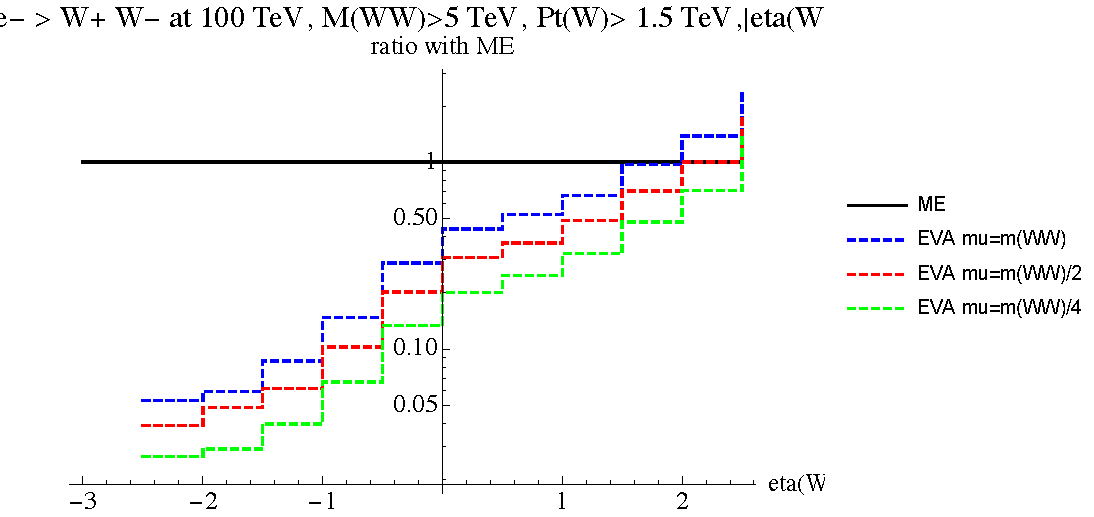
\includegraphics[width=0.46\linewidth]{Notebooks/PlotDistr/WW_WW/100TeVcuts/plotetaWratio2.pdf}
%\end{figure}

%\begin{figure}[ht]
%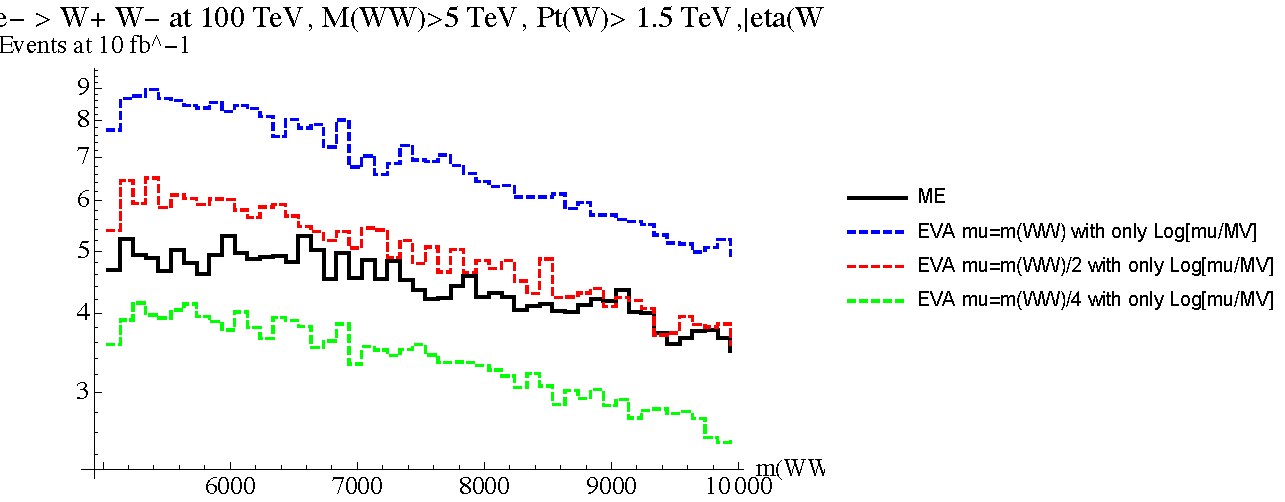
\includegraphics[width=0.46\linewidth]{Notebooks/PlotDistr/WW_WW/100TeVcuts/plotmWW.pdf}
%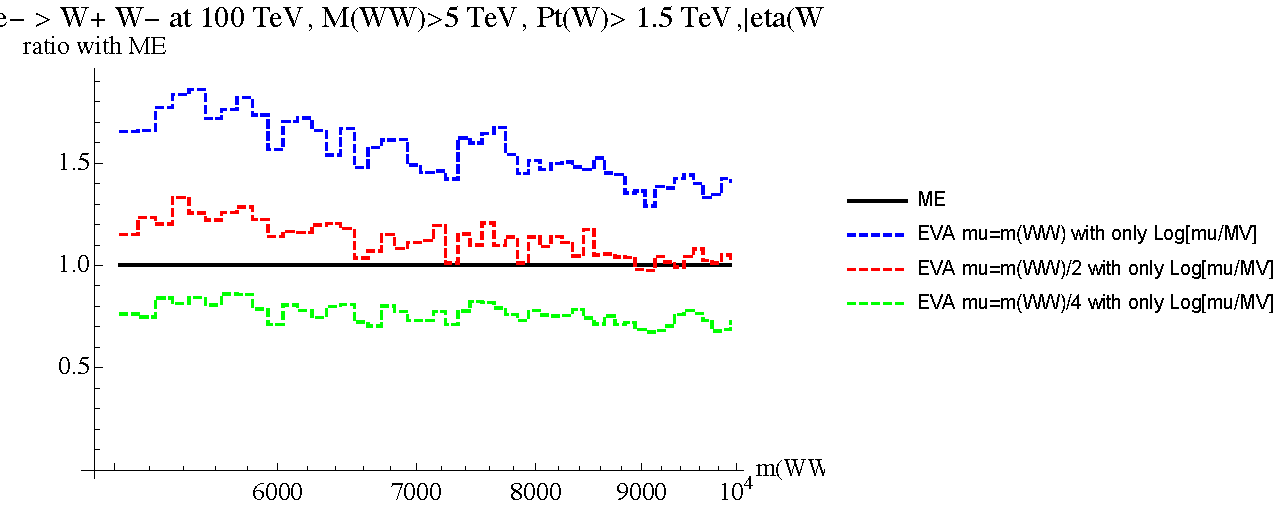
\includegraphics[width=0.46\linewidth]{Notebooks/PlotDistr/WW_WW/100TeVcuts/plotmWWratio1.pdf}
%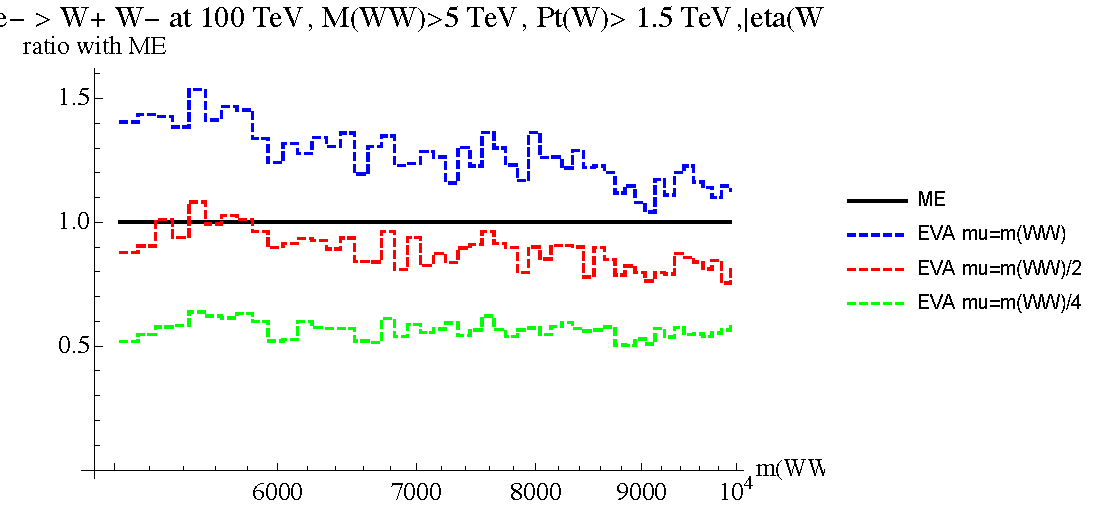
\includegraphics[width=0.46\linewidth]{Notebooks/PlotDistr/WW_WW/100TeVcuts/plotmWWratio2.pdf}
%\end{figure}

%\begin{figure}[ht]
%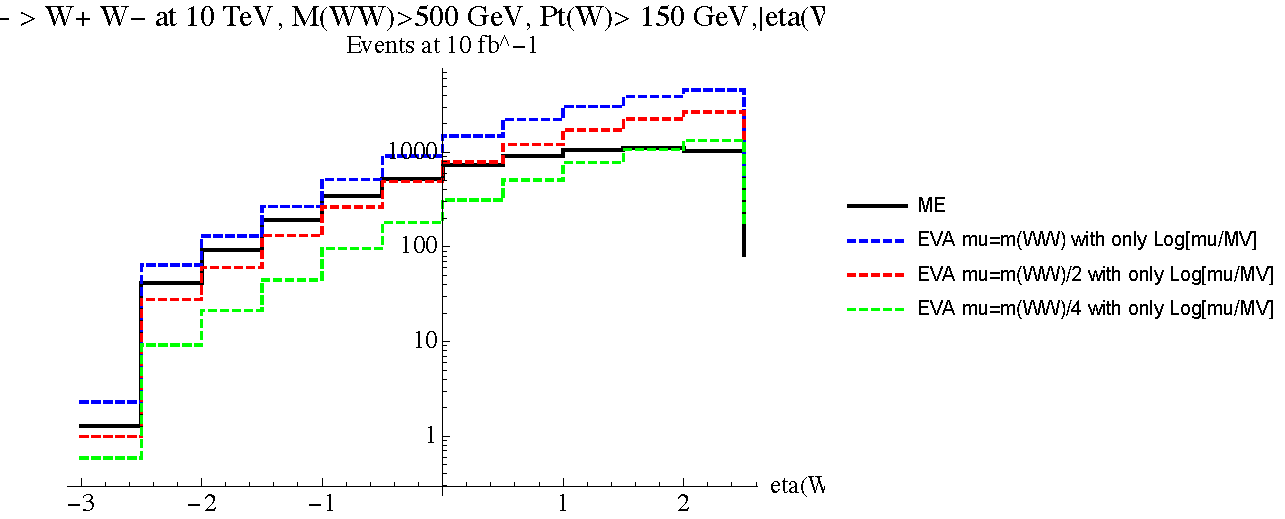
\includegraphics[width=0.46\linewidth]{Notebooks/PlotDistr/WW_WW/10TeVcuts/plotetaW.pdf}
%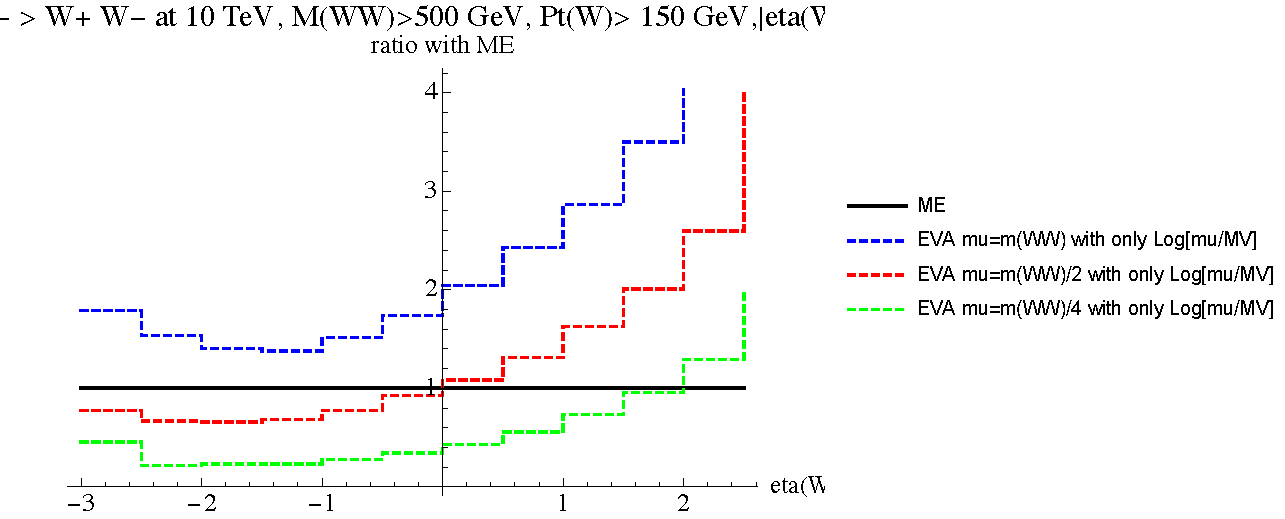
\includegraphics[width=0.46\linewidth]{Notebooks/PlotDistr/WW_WW/10TeVcuts/plotetaWratio1.pdf}
%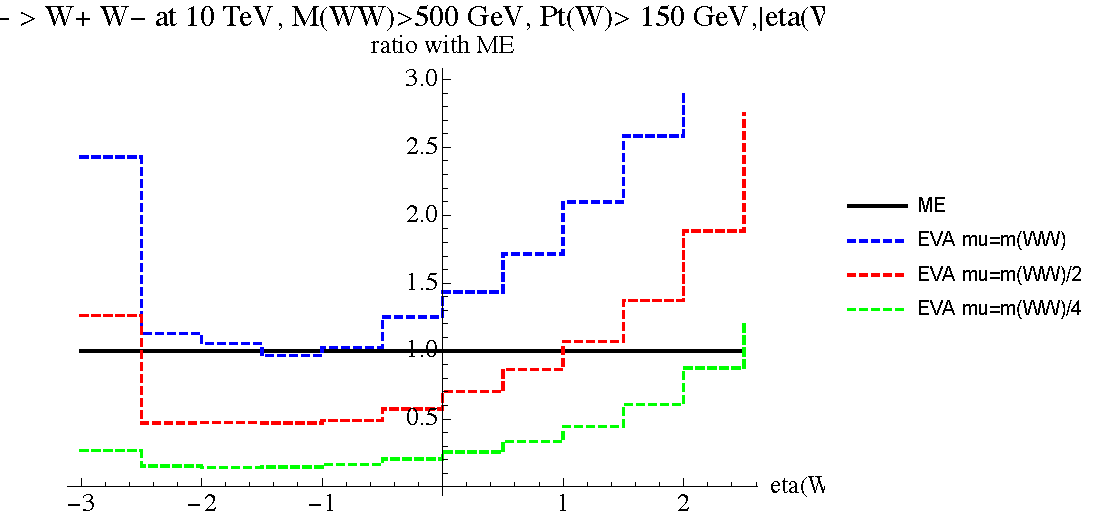
\includegraphics[width=0.46\linewidth]{Notebooks/PlotDistr/WW_WW/10TeVcuts/plotetaWratio2.pdf}
%\end{figure}

%\begin{figure}[ht]
%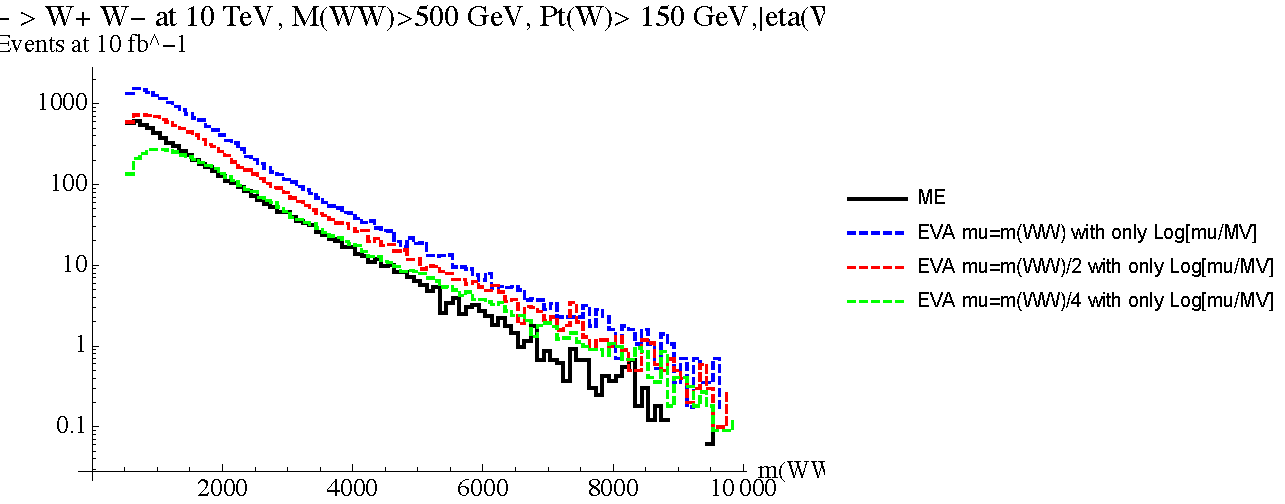
\includegraphics[width=0.46\linewidth]{Notebooks/PlotDistr/WW_WW/10TeVcuts/plotmWW.pdf}
%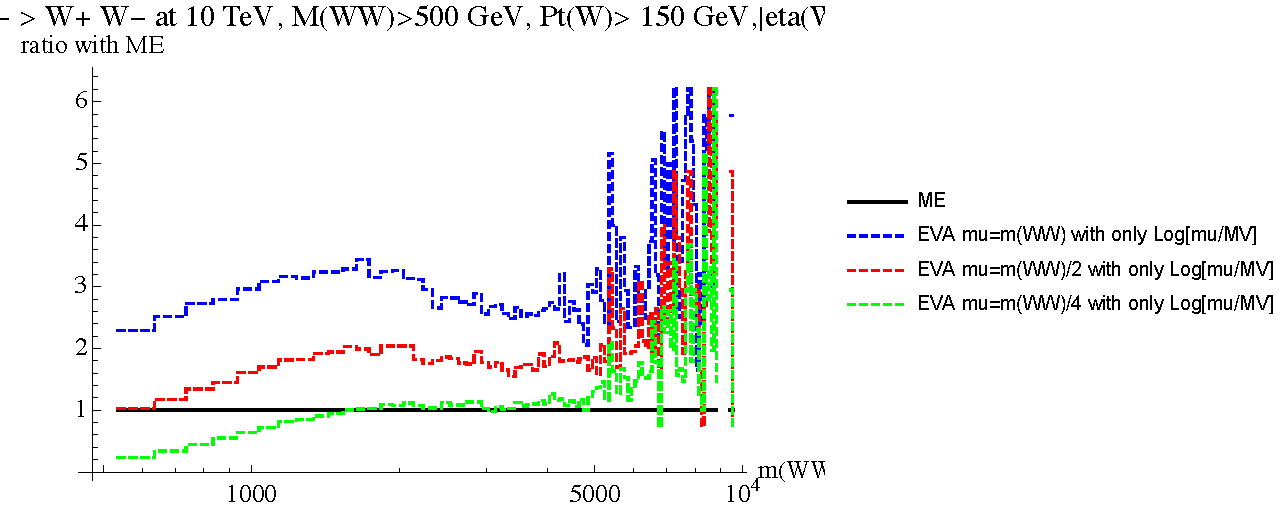
\includegraphics[width=0.46\linewidth]{Notebooks/PlotDistr/WW_WW/10TeVcuts/plotmWWratio1.pdf}
%\includegraphics[width=0.46\linewidth]{Notebooks/PlotDistr/WW_WW/10TeVcuts/plotmWWratio2.pdf}
%\end{figure}

%\begin{figure}[ht]
%\includegraphics[width=0.46\linewidth]{Notebooks/PlotDistr/WW_WW/10TeVolnlyptcut/plotetaW.pdf}
%\includegraphics[width=0.46\linewidth]{Notebooks/PlotDistr/WW_WW/10TeVolnlyptcut/plotetaWratio1.pdf}
%\includegraphics[width=0.46\linewidth]{Notebooks/PlotDistr/WW_WW/10TeVolnlyptcut/plotetaWratio2.pdf}
%\end{figure}

%\begin{figure}[ht]
%\includegraphics[width=0.46\linewidth]{Notebooks/PlotDistr/WW_WW/10TeVolnlyptcut/plotmWW.pdf}
%\includegraphics[width=0.46\linewidth]{Notebooks/PlotDistr/WW_WW/10TeVolnlyptcut/plotmWWratio1.pdf}
%\includegraphics[width=0.46\linewidth]{Notebooks/PlotDistr/WW_WW/10TeVolnlyptcut/plotmWWratio2.pdf}
%\end{figure}

\clearpage
\subsection{$WW$ into $t \bar t$}

%\begin{figure}[ht]
%\includegraphics[width=0.46\linewidth]{Notebooks/PlotDistr/WW_tt/10TeVcuts/plotetat.pdf}
%\includegraphics[width=0.46\linewidth]{Notebooks/PlotDistr/WW_tt/10TeVcuts/plotetatratio1.pdf}
%\includegraphics[width=0.46\linewidth]{Notebooks/PlotDistr/WW_tt/10TeVcuts/plotetatratio2.pdf}
%\end{figure}

%\begin{figure}[ht]
%\includegraphics[width=0.46\linewidth]{Notebooks/PlotDistr/WW_tt/10TeVcuts/plotmtt.pdf}
%\includegraphics[width=0.46\linewidth]{Notebooks/PlotDistr/WW_tt/10TeVcuts/plotmttratio1.pdf}
%\includegraphics[width=0.46\linewidth]{Notebooks/PlotDistr/WW_tt/10TeVcuts/plotmttratio2.pdf}
%\end{figure}

%\begin{figure}[ht]
%\includegraphics[width=0.46\linewidth]{Notebooks/PlotDistr/WW_tt/10TeVnocuts/plotetat.pdf}
%\includegraphics[width=0.46\linewidth]{Notebooks/PlotDistr/WW_tt/10TeVnocuts/plotetatratio1.pdf}
%\includegraphics[width=0.46\linewidth]{Notebooks/PlotDistr/WW_tt/10TeVnocuts/plotetatratio2.pdf}
%\end{figure}

%\begin{figure}[ht]
%\includegraphics[width=0.46\linewidth]{Notebooks/PlotDistr/WW_tt/10TeVnocuts/plotmtt.pdf}
%\includegraphics[width=0.46\linewidth]{Notebooks/PlotDistr/WW_tt/10TeVnocuts/plotmttratio1.pdf}
%\includegraphics[width=0.46\linewidth]{Notebooks/PlotDistr/WW_tt/10TeVnocuts/plotmttratio2.pdf}
%\end{figure}

\clearpage
\subsection{$ZZ$ into $t \bar t$}

%\begin{figure}[ht]
%\includegraphics[width=0.46\linewidth]{Notebooks/PlotDistr/ZZ_tt/10TeVcuts/plotetat.pdf}
%\includegraphics[width=0.46\linewidth]{Notebooks/PlotDistr/ZZ_tt/10TeVcuts/plotetatratio1.pdf}
%\includegraphics[width=0.46\linewidth]{Notebooks/PlotDistr/ZZ_tt/10TeVcuts/plotetatratio2.pdf}
%\end{figure}

%\begin{figure}[ht]
%\includegraphics[width=0.46\linewidth]{Notebooks/PlotDistr/ZZ_tt/10TeVcuts/plotmtt.pdf}
%\includegraphics[width=0.46\linewidth]{Notebooks/PlotDistr/ZZ_tt/10TeVcuts/plotmttratio1.pdf}
%\includegraphics[width=0.46\linewidth]{Notebooks/PlotDistr/ZZ_tt/10TeVcuts/plotmttratio2.pdf}
%\end{figure}

%\begin{figure}[ht]
%\includegraphics[width=0.46\linewidth]{Notebooks/PlotDistr/ZZ_tt/10TeVnocuts/plotetat.pdf}
%\includegraphics[width=0.46\linewidth]{Notebooks/PlotDistr/ZZ_tt/10TeVnocuts/plotetatratio1.pdf}
%\includegraphics[width=0.46\linewidth]{Notebooks/PlotDistr/ZZ_tt/10TeVnocuts/plotetatratio2.pdf}
%\end{figure}

%\begin{figure}[ht]
%\includegraphics[width=0.46\linewidth]{Notebooks/PlotDistr/ZZ_tt/10TeVnocuts/plotmtt.pdf}
%\includegraphics[width=0.46\linewidth]{Notebooks/PlotDistr/ZZ_tt/10TeVnocuts/plotmttratio1.pdf}
%\includegraphics[width=0.46\linewidth]{Notebooks/PlotDistr/ZZ_tt/10TeVnocuts/plotmttratio2.pdf}
%\end{figure}

%%\begin{figure}[ht]
%%\includegraphics[width=0.46\linewidth]{Notebooks/PlotLumi/10TeV/lumis/WmL-WpL.pdf}
%%\includegraphics[width=0.46\linewidth]{Notebooks/PlotLumi/10TeV/lumis/WmL-WpT.pdf}
%%\includegraphics[width=0.46\linewidth]{Notebooks/PlotLumi/10TeV/lumis/WmT-WpL.pdf}
%%\includegraphics[width=0.46\linewidth]{Notebooks/PlotLumi/10TeV/lumis/WmT-WpT.pdf}
%%\includegraphics[width=0.46\linewidth]{Notebooks/PlotLumi/10TeV/lumis/Wmm-Wpm.pdf}
%%\includegraphics[width=0.46\linewidth]{Notebooks/PlotLumi/10TeV/lumis/Wmm-Wpp.pdf}
%%\end{figure}
%
%%\begin{figure}[ht]
%%\includegraphics[width=0.46\linewidth]{Notebooks/PlotLumi/10TeV/lumis/Wmp-Wpm.pdf}
%%\includegraphics[width=0.46\linewidth]{Notebooks/PlotLumi/10TeV/lumis/Wmp-Wpp.pdf}
%%\includegraphics[width=0.46\linewidth]{Notebooks/PlotLumi/10TeV/lumis/ZL-ZL.pdf}
%%\includegraphics[width=0.46\linewidth]{Notebooks/PlotLumi/10TeV/lumis/ZL-ZT.pdf}
%%\includegraphics[width=0.46\linewidth]{Notebooks/PlotLumi/10TeV/lumis/ZT-ZL.pdf}
%%\includegraphics[width=0.46\linewidth]{Notebooks/PlotLumi/10TeV/lumis/ZT-ZT.pdf}
%%\end{figure}
%
%%\begin{figure}[ht]
%%\includegraphics[width=0.46\linewidth]{Notebooks/PlotLumi/10TeV/lumis/Zm-Zm.pdf}
%%\includegraphics[width=0.46\linewidth]{Notebooks/PlotLumi/10TeV/lumis/Zp-Zm.pdf}
%%\includegraphics[width=0.46\linewidth]{Notebooks/PlotLumi/10TeV/lumis/Zp-Zp.pdf}
%%\end{figure}
%

\clearpage
\section{Luminosities}

\subsection{10 TeV}

%\begin{figure}[ht]
%\includegraphics[width=0.46\linewidth]{Notebooks/PlotLumi/10TeV/lumis/plotWWpolRandL.pdf}
%\includegraphics[width=0.46\linewidth]{Notebooks/PlotLumi/10TeV/lumis/plotWWpolTand0.pdf}
%\includegraphics[width=0.46\linewidth]{Notebooks/PlotLumi/10TeV/lumis/plotWmWpandWpWm.pdf}
%\includegraphics[width=0.46\linewidth]{Notebooks/PlotLumi/10TeV/lumis/plotZZpolRandL.pdf}
%\includegraphics[width=0.46\linewidth]{Notebooks/PlotLumi/10TeV/lumis/plotZZpolTand0.pdf}
%\end{figure}

%\begin{figure}
%\includegraphics[width=0.46\linewidth]{Notebooks/PlotLumi/10TeV/lumis/plotgammaWZ.pdf}
%\end{figure}

\clearpage
\subsubsection{Comparisons with EVAs}

%\begin{figure}[ht]
%\includegraphics[width=0.46\linewidth]{Notebooks/PlotLumi/10TeV/ratios/WmL-WpL.pdf}
%\includegraphics[width=0.46\linewidth]{Notebooks/PlotLumi/10TeV/ratios/WmL-WpT.pdf}
%\includegraphics[width=0.46\linewidth]{Notebooks/PlotLumi/10TeV/ratios/WmT-WpL.pdf}
%\includegraphics[width=0.46\linewidth]{Notebooks/PlotLumi/10TeV/ratios/WmT-WpT.pdf}
%\includegraphics[width=0.46\linewidth]{Notebooks/PlotLumi/10TeV/ratios/Wmm-Wpm.pdf}
%\includegraphics[width=0.46\linewidth]{Notebooks/PlotLumi/10TeV/ratios/Wmm-Wpp.pdf}
%\end{figure}

%\begin{figure}[ht]
%\includegraphics[width=0.46\linewidth]{Notebooks/PlotLumi/10TeV/ratios/Wmp-Wpm.pdf}
%\includegraphics[width=0.46\linewidth]{Notebooks/PlotLumi/10TeV/ratios/Wmp-Wpp.pdf}
%\includegraphics[width=0.46\linewidth]{Notebooks/PlotLumi/10TeV/ratios/ZL-ZL.pdf}
%\includegraphics[width=0.46\linewidth]{Notebooks/PlotLumi/10TeV/ratios/ZL-ZT.pdf}
%\includegraphics[width=0.46\linewidth]{Notebooks/PlotLumi/10TeV/ratios/ZT-ZL.pdf}
%\includegraphics[width=0.46\linewidth]{Notebooks/PlotLumi/10TeV/ratios/ZT-ZT.pdf}
%\end{figure}

%\begin{figure}[ht]
%\includegraphics[width=0.46\linewidth]{Notebooks/PlotLumi/10TeV/ratios/Zm-Zm.pdf}
%\includegraphics[width=0.46\linewidth]{Notebooks/PlotLumi/10TeV/ratios/Zp-Zm.pdf}
%\includegraphics[width=0.46\linewidth]{Notebooks/PlotLumi/10TeV/ratios/Zp-Zp.pdf}
%\end{figure}

%%\begin{figure}[ht]
%%\includegraphics[width=0.46\linewidth]{Notebooks/PlotLumi/1TeV/lumis/WmL-WpL.pdf}
%%\includegraphics[width=0.46\linewidth]{Notebooks/PlotLumi/1TeV/lumis/WmL-WpT.pdf}
%%\includegraphics[width=0.46\linewidth]{Notebooks/PlotLumi/1TeV/lumis/WmT-WpL.pdf}
%%\includegraphics[width=0.46\linewidth]{Notebooks/PlotLumi/1TeV/lumis/WmT-WpT.pdf}
%%\includegraphics[width=0.46\linewidth]{Notebooks/PlotLumi/1TeV/lumis/Wmm-Wpm.pdf}
%%\includegraphics[width=0.46\linewidth]{Notebooks/PlotLumi/1TeV/lumis/Wmm-Wpp.pdf}
%%\end{figure}
%
%%\begin{figure}[ht]
%%\includegraphics[width=0.46\linewidth]{Notebooks/PlotLumi/1TeV/lumis/Wmp-Wpm.pdf}
%%\includegraphics[width=0.46\linewidth]{Notebooks/PlotLumi/1TeV/lumis/Wmp-Wpp.pdf}
%%\includegraphics[width=0.46\linewidth]{Notebooks/PlotLumi/1TeV/lumis/ZL-ZL.pdf}
%%\includegraphics[width=0.46\linewidth]{Notebooks/PlotLumi/1TeV/lumis/ZL-ZT.pdf}
%%\includegraphics[width=0.46\linewidth]{Notebooks/PlotLumi/1TeV/lumis/ZT-ZL.pdf}
%%\includegraphics[width=0.46\linewidth]{Notebooks/PlotLumi/1TeV/lumis/ZT-ZT.pdf}
%%\end{figure}
%
%%\begin{figure}[ht]
%%\includegraphics[width=0.46\linewidth]{Notebooks/PlotLumi/1TeV/lumis/Zm-Zm.pdf}
%%\includegraphics[width=0.46\linewidth]{Notebooks/PlotLumi/1TeV/lumis/Zp-Zm.pdf}
%%\includegraphics[width=0.46\linewidth]{Notebooks/PlotLumi/1TeV/lumis/Zp-Zp.pdf}
%%\end{figure}
%
\clearpage
\subsection{1 TeV}

%\begin{figure}[ht]
%\includegraphics[width=0.46\linewidth]{Notebooks/PlotLumi/1TeV/lumis/plotWWpolRandL.pdf}
%\includegraphics[width=0.46\linewidth]{Notebooks/PlotLumi/1TeV/lumis/plotWWpolTand0.pdf}
%\includegraphics[width=0.46\linewidth]{Notebooks/PlotLumi/1TeV/lumis/plotWmWpandWpWm.pdf}
%\includegraphics[width=0.46\linewidth]{Notebooks/PlotLumi/1TeV/lumis/plotZZpolRandL.pdf}
%\includegraphics[width=0.46\linewidth]{Notebooks/PlotLumi/1TeV/lumis/plotZZpolTand0.pdf}
%\end{figure}

%\begin{figure}
%\includegraphics[width=0.46\linewidth]{Notebooks/PlotLumi/1TeV/lumis/plotgammaWZ.pdf}
%\end{figure}

\clearpage
\subsubsection{Comparisons with EVAs}


%\begin{figure}[ht]
%\includegraphics[width=0.46\linewidth]{Notebooks/PlotLumi/1TeV/ratios/WmL-WpL.pdf}
%\includegraphics[width=0.46\linewidth]{Notebooks/PlotLumi/1TeV/ratios/WmL-WpT.pdf}
%\includegraphics[width=0.46\linewidth]{Notebooks/PlotLumi/1TeV/ratios/WmT-WpL.pdf}
%\includegraphics[width=0.46\linewidth]{Notebooks/PlotLumi/1TeV/ratios/WmT-WpT.pdf}
%\includegraphics[width=0.46\linewidth]{Notebooks/PlotLumi/1TeV/ratios/Wmm-Wpm.pdf}
%\includegraphics[width=0.46\linewidth]{Notebooks/PlotLumi/1TeV/ratios/Wmm-Wpp.pdf}
%\end{figure}

%\begin{figure}[ht]
%\includegraphics[width=0.46\linewidth]{Notebooks/PlotLumi/1TeV/ratios/Wmp-Wpm.pdf}
%\includegraphics[width=0.46\linewidth]{Notebooks/PlotLumi/1TeV/ratios/Wmp-Wpp.pdf}
%\includegraphics[width=0.46\linewidth]{Notebooks/PlotLumi/1TeV/ratios/ZL-ZL.pdf}
%\includegraphics[width=0.46\linewidth]{Notebooks/PlotLumi/1TeV/ratios/ZL-ZT.pdf}
%\includegraphics[width=0.46\linewidth]{Notebooks/PlotLumi/1TeV/ratios/ZT-ZL.pdf}
%\includegraphics[width=0.46\linewidth]{Notebooks/PlotLumi/1TeV/ratios/ZT-ZT.pdf}
%\end{figure}

%\begin{figure}[ht]
%\includegraphics[width=0.46\linewidth]{Notebooks/PlotLumi/1TeV/ratios/Zm-Zm.pdf}
%\includegraphics[width=0.46\linewidth]{Notebooks/PlotLumi/1TeV/ratios/Zp-Zm.pdf}
%\includegraphics[width=0.46\linewidth]{Notebooks/PlotLumi/1TeV/ratios/Zp-Zp.pdf}
%\end{figure}

%%\begin{figure}[ht]
%%\includegraphics[width=0.46\linewidth]{Notebooks/PlotLumi/30TeV/lumis/WmL-WpL.pdf}
%%\includegraphics[width=0.46\linewidth]{Notebooks/PlotLumi/30TeV/lumis/WmL-WpT.pdf}
%%\includegraphics[width=0.46\linewidth]{Notebooks/PlotLumi/30TeV/lumis/WmT-WpL.pdf}
%%\includegraphics[width=0.46\linewidth]{Notebooks/PlotLumi/30TeV/lumis/WmT-WpT.pdf}
%%\includegraphics[width=0.46\linewidth]{Notebooks/PlotLumi/30TeV/lumis/Wmm-Wpm.pdf}
%%\includegraphics[width=0.46\linewidth]{Notebooks/PlotLumi/30TeV/lumis/Wmm-Wpp.pdf}
%%\end{figure}
%
%%\begin{figure}[ht]
%%\includegraphics[width=0.46\linewidth]{Notebooks/PlotLumi/30TeV/lumis/Wmp-Wpm.pdf}
%%\includegraphics[width=0.46\linewidth]{Notebooks/PlotLumi/30TeV/lumis/Wmp-Wpp.pdf}
%%\includegraphics[width=0.46\linewidth]{Notebooks/PlotLumi/30TeV/lumis/ZL-ZL.pdf}
%%\includegraphics[width=0.46\linewidth]{Notebooks/PlotLumi/30TeV/lumis/ZL-ZT.pdf}
%%\includegraphics[width=0.46\linewidth]{Notebooks/PlotLumi/30TeV/lumis/ZT-ZL.pdf}
%%\includegraphics[width=0.46\linewidth]{Notebooks/PlotLumi/30TeV/lumis/ZT-ZT.pdf}
%%\end{figure}
%
%%\begin{figure}[ht]
%%\includegraphics[width=0.46\linewidth]{Notebooks/PlotLumi/30TeV/lumis/Zm-Zm.pdf}
%%\includegraphics[width=0.46\linewidth]{Notebooks/PlotLumi/30TeV/lumis/Zp-Zm.pdf}
%%\includegraphics[width=0.46\linewidth]{Notebooks/PlotLumi/30TeV/lumis/Zp-Zp.pdf}
%%\end{figure}
%

\clearpage
\subsection{30 TeV}

%\begin{figure}[ht]
%\includegraphics[width=0.46\linewidth]{Notebooks/PlotLumi/30TeV/lumis/plotWWpolRandL.pdf}
%\includegraphics[width=0.46\linewidth]{Notebooks/PlotLumi/30TeV/lumis/plotWWpolTand0.pdf}
%\includegraphics[width=0.46\linewidth]{Notebooks/PlotLumi/30TeV/lumis/plotWmWpandWpWm.pdf}
%\includegraphics[width=0.46\linewidth]{Notebooks/PlotLumi/30TeV/lumis/plotZZpolRandL.pdf}
%\includegraphics[width=0.46\linewidth]{Notebooks/PlotLumi/30TeV/lumis/plotZZpolTand0.pdf}
%\end{figure}

%\begin{figure}
%\includegraphics[width=0.46\linewidth]{Notebooks/PlotLumi/30TeV/lumis/plotgammaWZ.pdf}
%\end{figure}

\clearpage
\subsubsection{Comparisons with EVAs}


%\begin{figure}[ht]
%\includegraphics[width=0.46\linewidth]{Notebooks/PlotLumi/30TeV/ratios/WmL-WpL.pdf}
%\includegraphics[width=0.46\linewidth]{Notebooks/PlotLumi/30TeV/ratios/WmL-WpT.pdf}
%\includegraphics[width=0.46\linewidth]{Notebooks/PlotLumi/30TeV/ratios/WmT-WpL.pdf}
%\includegraphics[width=0.46\linewidth]{Notebooks/PlotLumi/30TeV/ratios/WmT-WpT.pdf}
%\includegraphics[width=0.46\linewidth]{Notebooks/PlotLumi/30TeV/ratios/Wmm-Wpm.pdf}
%\includegraphics[width=0.46\linewidth]{Notebooks/PlotLumi/30TeV/ratios/Wmm-Wpp.pdf}
%\end{figure}

%\begin{figure}[ht]
%\includegraphics[width=0.46\linewidth]{Notebooks/PlotLumi/30TeV/ratios/Wmp-Wpm.pdf}
%\includegraphics[width=0.46\linewidth]{Notebooks/PlotLumi/30TeV/ratios/Wmp-Wpp.pdf}
%\includegraphics[width=0.46\linewidth]{Notebooks/PlotLumi/30TeV/ratios/ZL-ZL.pdf}
%\includegraphics[width=0.46\linewidth]{Notebooks/PlotLumi/30TeV/ratios/ZL-ZT.pdf}
%\includegraphics[width=0.46\linewidth]{Notebooks/PlotLumi/30TeV/ratios/ZT-ZL.pdf}
%\includegraphics[width=0.46\linewidth]{Notebooks/PlotLumi/30TeV/ratios/ZT-ZT.pdf}
%\end{figure}

%\begin{figure}[ht]
%\includegraphics[width=0.46\linewidth]{Notebooks/PlotLumi/30TeV/ratios/Zm-Zm.pdf}
%\includegraphics[width=0.46\linewidth]{Notebooks/PlotLumi/30TeV/ratios/Zp-Zm.pdf}
%\includegraphics[width=0.46\linewidth]{Notebooks/PlotLumi/30TeV/ratios/Zp-Zp.pdf}
%\end{figure}

%%\begin{figure}[ht]
%%\includegraphics[width=0.46\linewidth]{Notebooks/PlotLumi/3TeV/lumis/WmL-WpL.pdf}
%%\includegraphics[width=0.46\linewidth]{Notebooks/PlotLumi/3TeV/lumis/WmL-WpT.pdf}
%%\includegraphics[width=0.46\linewidth]{Notebooks/PlotLumi/3TeV/lumis/WmT-WpL.pdf}
%%\includegraphics[width=0.46\linewidth]{Notebooks/PlotLumi/3TeV/lumis/WmT-WpT.pdf}
%%\includegraphics[width=0.46\linewidth]{Notebooks/PlotLumi/3TeV/lumis/Wmm-Wpm.pdf}
%%\includegraphics[width=0.46\linewidth]{Notebooks/PlotLumi/3TeV/lumis/Wmm-Wpp.pdf}
%%\end{figure}
%
%%\begin{figure}[ht]
%%\includegraphics[width=0.46\linewidth]{Notebooks/PlotLumi/3TeV/lumis/Wmp-Wpm.pdf}
%%\includegraphics[width=0.46\linewidth]{Notebooks/PlotLumi/3TeV/lumis/Wmp-Wpp.pdf}
%%\includegraphics[width=0.46\linewidth]{Notebooks/PlotLumi/3TeV/lumis/ZL-ZL.pdf}
%%\includegraphics[width=0.46\linewidth]{Notebooks/PlotLumi/3TeV/lumis/ZL-ZT.pdf}
%%\includegraphics[width=0.46\linewidth]{Notebooks/PlotLumi/3TeV/lumis/ZT-ZL.pdf}
%%\includegraphics[width=0.46\linewidth]{Notebooks/PlotLumi/3TeV/lumis/ZT-ZT.pdf}
%%\end{figure}
%
%%\begin{figure}[ht]
%%\includegraphics[width=0.46\linewidth]{Notebooks/PlotLumi/3TeV/lumis/Zm-Zm.pdf}
%%\includegraphics[width=0.46\linewidth]{Notebooks/PlotLumi/3TeV/lumis/Zp-Zm.pdf}
%%\includegraphics[width=0.46\linewidth]{Notebooks/PlotLumi/3TeV/lumis/Zp-Zp.pdf}
%%\end{figure}

\clearpage
\subsection{3 TeV}

%\begin{figure}[ht]
%\includegraphics[width=0.46\linewidth]{Notebooks/PlotLumi/3TeV/lumis/plotWWpolRandL.pdf}
%\includegraphics[width=0.46\linewidth]{Notebooks/PlotLumi/3TeV/lumis/plotWWpolTand0.pdf}
%\includegraphics[width=0.46\linewidth]{Notebooks/PlotLumi/3TeV/lumis/plotWmWpandWpWm.pdf}
%\includegraphics[width=0.46\linewidth]{Notebooks/PlotLumi/3TeV/lumis/plotZZpolRandL.pdf}
%\includegraphics[width=0.46\linewidth]{Notebooks/PlotLumi/3TeV/lumis/plotZZpolTand0.pdf}
%\end{figure}

%\begin{figure}
%\includegraphics[width=0.46\linewidth]{Notebooks/PlotLumi/3TeV/lumis/plotgammaWZ.pdf}
%\end{figure}


\clearpage
\subsubsection{Comparisons with EVAs}



%\begin{figure}[ht]
%\includegraphics[width=0.46\linewidth]{Notebooks/PlotLumi/3TeV/ratios/WmL-WpL.pdf}
%\includegraphics[width=0.46\linewidth]{Notebooks/PlotLumi/3TeV/ratios/WmL-WpT.pdf}
%\includegraphics[width=0.46\linewidth]{Notebooks/PlotLumi/3TeV/ratios/WmT-WpL.pdf}
%\includegraphics[width=0.46\linewidth]{Notebooks/PlotLumi/3TeV/ratios/WmT-WpT.pdf}
%\includegraphics[width=0.46\linewidth]{Notebooks/PlotLumi/3TeV/ratios/Wmm-Wpm.pdf}
%\includegraphics[width=0.46\linewidth]{Notebooks/PlotLumi/3TeV/ratios/Wmm-Wpp.pdf}
%\end{figure}

%\begin{figure}[ht]
%\includegraphics[width=0.46\linewidth]{Notebooks/PlotLumi/3TeV/ratios/Wmp-Wpm.pdf}
%\includegraphics[width=0.46\linewidth]{Notebooks/PlotLumi/3TeV/ratios/Wmp-Wpp.pdf}
%\includegraphics[width=0.46\linewidth]{Notebooks/PlotLumi/3TeV/ratios/ZL-ZL.pdf}
%\includegraphics[width=0.46\linewidth]{Notebooks/PlotLumi/3TeV/ratios/ZL-ZT.pdf}
%\includegraphics[width=0.46\linewidth]{Notebooks/PlotLumi/3TeV/ratios/ZT-ZL.pdf}
%\includegraphics[width=0.46\linewidth]{Notebooks/PlotLumi/3TeV/ratios/ZT-ZT.pdf}
%\end{figure}

%\begin{figure}[ht]
%\includegraphics[width=0.46\linewidth]{Notebooks/PlotLumi/3TeV/ratios/Zm-Zm.pdf}
%\includegraphics[width=0.46\linewidth]{Notebooks/PlotLumi/3TeV/ratios/Zp-Zm.pdf}
%\includegraphics[width=0.46\linewidth]{Notebooks/PlotLumi/3TeV/ratios/Zp-Zp.pdf}
%\end{figure}



\clearpage
\section{PDFs vs EVA}

\subsection{All together, for $\mu+$ and $\mu-$ but same partons}

%\begin{figure}[ht]
%\includegraphics[width=0.46\linewidth]{Notebooks/PlotPDFs/alltogether/10TeV_mu+scaleQ.pdf}
%\includegraphics[width=0.46\linewidth]{Notebooks/PlotPDFs/alltogether/10TeV_mu+scaleQsqrtx.pdf}
%\includegraphics[width=0.46\linewidth]{Notebooks/PlotPDFs/alltogether/10TeV_mu+scaleQx.pdf}
%\end{figure}

%\begin{figure}[ht]
%\includegraphics[width=0.46\linewidth]{Notebooks/PlotPDFs/alltogether/10TeV_mu-scaleQ.pdf}
%\includegraphics[width=0.46\linewidth]{Notebooks/PlotPDFs/alltogether/10TeV_mu-scaleQsqrtx.pdf}
%\includegraphics[width=0.46\linewidth]{Notebooks/PlotPDFs/alltogether/10TeV_mu-scaleQx.pdf}
%\end{figure}

%\begin{figure}[ht]
%\includegraphics[width=0.46\linewidth]{Notebooks/PlotPDFs/alltogether/1TeV_mu+scaleQ.pdf}
%\includegraphics[width=0.46\linewidth]{Notebooks/PlotPDFs/alltogether/1TeV_mu+scaleQsqrtx.pdf}
%\includegraphics[width=0.46\linewidth]{Notebooks/PlotPDFs/alltogether/1TeV_mu+scaleQx.pdf}
%\end{figure}


%\begin{figure}[ht]
%\includegraphics[width=0.46\linewidth]{Notebooks/PlotPDFs/alltogether/1TeV_mu-scaleQ.pdf}
%\includegraphics[width=0.46\linewidth]{Notebooks/PlotPDFs/alltogether/1TeV_mu-scaleQsqrtx.pdf}
%\includegraphics[width=0.46\linewidth]{Notebooks/PlotPDFs/alltogether/1TeV_mu-scaleQx.pdf}
%\end{figure}

%\begin{figure}[ht]
%\includegraphics[width=0.46\linewidth]{Notebooks/PlotPDFs/alltogether/30TeV_mu+scaleQ.pdf}
%\includegraphics[width=0.46\linewidth]{Notebooks/PlotPDFs/alltogether/30TeV_mu+scaleQsqrtx.pdf}
%\includegraphics[width=0.46\linewidth]{Notebooks/PlotPDFs/alltogether/30TeV_mu+scaleQx.pdf}
%\end{figure}

%\begin{figure}[ht]
%\includegraphics[width=0.46\linewidth]{Notebooks/PlotPDFs/alltogether/30TeV_mu-scaleQ.pdf}
%\includegraphics[width=0.46\linewidth]{Notebooks/PlotPDFs/alltogether/30TeV_mu-scaleQsqrtx.pdf}
%\includegraphics[width=0.46\linewidth]{Notebooks/PlotPDFs/alltogether/30TeV_mu-scaleQx.pdf}
%\end{figure}

%\begin{figure}[ht]
%\includegraphics[width=0.46\linewidth]{Notebooks/PlotPDFs/alltogether/3TeV_mu+scaleQ.pdf}
%\includegraphics[width=0.46\linewidth]{Notebooks/PlotPDFs/alltogether/3TeV_mu+scaleQsqrtx.pdf}
%\includegraphics[width=0.46\linewidth]{Notebooks/PlotPDFs/alltogether/3TeV_mu+scaleQx.pdf}
%\end{figure}

%\begin{figure}[ht]
%\includegraphics[width=0.46\linewidth]{Notebooks/PlotPDFs/alltogether/3TeV_mu-scaleQ.pdf}
%\includegraphics[width=0.46\linewidth]{Notebooks/PlotPDFs/alltogether/3TeV_mu-scaleQsqrtx.pdf}
%\includegraphics[width=0.46\linewidth]{Notebooks/PlotPDFs/alltogether/3TeV_mu-scaleQx.pdf}
%\end{figure}



\clearpage
\subsection{Individuals PDF vs EVAs 10 TeV}

%\begin{figure}[ht]
%\includegraphics[width=0.46\linewidth]{Notebooks/PlotPDFs/ratios/10TeV/W-_0_Q.pdf}
%\includegraphics[width=0.46\linewidth]{Notebooks/PlotPDFs/ratios/10TeV/W-_0_Qsqrtx.pdf}
%\includegraphics[width=0.46\linewidth]{Notebooks/PlotPDFs/ratios/10TeV/W-_0_Qx.pdf}
%\end{figure}

%\begin{figure}[ht]
%\includegraphics[width=0.46\linewidth]{Notebooks/PlotPDFs/ratios/10TeV/W-_L_Q.pdf}
%\includegraphics[width=0.46\linewidth]{Notebooks/PlotPDFs/ratios/10TeV/W-_L_Qsqrtx.pdf}
%\includegraphics[width=0.46\linewidth]{Notebooks/PlotPDFs/ratios/10TeV/W-_L_Qx.pdf}
%\end{figure}

%\begin{figure}[ht]
%\includegraphics[width=0.46\linewidth]{Notebooks/PlotPDFs/ratios/10TeV/W-_R_Q.pdf}
%\includegraphics[width=0.46\linewidth]{Notebooks/PlotPDFs/ratios/10TeV/W-_R_Qsqrtx.pdf}
%\includegraphics[width=0.46\linewidth]{Notebooks/PlotPDFs/ratios/10TeV/W-_R_Qx.pdf}
%\end{figure}

%\begin{figure}[ht]
%\includegraphics[width=0.46\linewidth]{Notebooks/PlotPDFs/ratios/10TeV/W-_T_Q.pdf}
%\includegraphics[width=0.46\linewidth]{Notebooks/PlotPDFs/ratios/10TeV/W-_T_Qsqrtx.pdf}
%\includegraphics[width=0.46\linewidth]{Notebooks/PlotPDFs/ratios/10TeV/W-_T_Qx.pdf}
%\end{figure}

%\begin{figure}[ht]
%\includegraphics[width=0.46\linewidth]{Notebooks/PlotPDFs/ratios/10TeV/Z_0_Q.pdf}
%\includegraphics[width=0.46\linewidth]{Notebooks/PlotPDFs/ratios/10TeV/Z_0_Qsqrtx.pdf}
%\includegraphics[width=0.46\linewidth]{Notebooks/PlotPDFs/ratios/10TeV/Z_0_Qx.pdf}
%\end{figure}

%\begin{figure}[ht]
%\includegraphics[width=0.46\linewidth]{Notebooks/PlotPDFs/ratios/10TeV/Z_L-_Q.pdf}
%\includegraphics[width=0.46\linewidth]{Notebooks/PlotPDFs/ratios/10TeV/Z_L-_Qsqrtx.pdf}
%\includegraphics[width=0.46\linewidth]{Notebooks/PlotPDFs/ratios/10TeV/Z_L-_Qx.pdf}
%\end{figure}

%\begin{figure}[ht]
%\includegraphics[width=0.46\linewidth]{Notebooks/PlotPDFs/ratios/10TeV/Z_R_Q.pdf}
%\includegraphics[width=0.46\linewidth]{Notebooks/PlotPDFs/ratios/10TeV/Z_R_Qsqrtx.pdf}
%\includegraphics[width=0.46\linewidth]{Notebooks/PlotPDFs/ratios/10TeV/Z_R_Qx.pdf}
%\end{figure}

%\begin{figure}[ht]
%\includegraphics[width=0.46\linewidth]{Notebooks/PlotPDFs/ratios/10TeV/Z_T_Q.pdf}
%\includegraphics[width=0.46\linewidth]{Notebooks/PlotPDFs/ratios/10TeV/Z_T_Qsqrtx.pdf}
%\includegraphics[width=0.46\linewidth]{Notebooks/PlotPDFs/ratios/10TeV/Z_T_Qx.pdf}
%\end{figure}

%\begin{figure}[ht]
%\includegraphics[width=0.46\linewidth]{Notebooks/PlotPDFs/ratios/1TeV/W-_0_Q.pdf}
%\includegraphics[width=0.46\linewidth]{Notebooks/PlotPDFs/ratios/1TeV/W-_0_Qsqrtx.pdf}
%\includegraphics[width=0.46\linewidth]{Notebooks/PlotPDFs/ratios/1TeV/W-_0_Qx.pdf}
%\end{figure}

\clearpage
\subsection{Individuals PDF vs EVAs 1 TeV}

%\begin{figure}[ht]
%\includegraphics[width=0.46\linewidth]{Notebooks/PlotPDFs/ratios/1TeV/W-_L_Q.pdf}
%\includegraphics[width=0.46\linewidth]{Notebooks/PlotPDFs/ratios/1TeV/W-_L_Qsqrtx.pdf}
%\includegraphics[width=0.46\linewidth]{Notebooks/PlotPDFs/ratios/1TeV/W-_L_Qx.pdf}
%\end{figure}

%\begin{figure}[ht]
%\includegraphics[width=0.46\linewidth]{Notebooks/PlotPDFs/ratios/1TeV/W-_R_Q.pdf}
%\includegraphics[width=0.46\linewidth]{Notebooks/PlotPDFs/ratios/1TeV/W-_R_Qsqrtx.pdf}
%\includegraphics[width=0.46\linewidth]{Notebooks/PlotPDFs/ratios/1TeV/W-_R_Qx.pdf}
%\end{figure}

%\begin{figure}[ht]
%\includegraphics[width=0.46\linewidth]{Notebooks/PlotPDFs/ratios/1TeV/W-_T_Q.pdf}
%\includegraphics[width=0.46\linewidth]{Notebooks/PlotPDFs/ratios/1TeV/W-_T_Qsqrtx.pdf}
%\includegraphics[width=0.46\linewidth]{Notebooks/PlotPDFs/ratios/1TeV/W-_T_Qx.pdf}
%\end{figure}

%\begin{figure}[ht]
%\includegraphics[width=0.46\linewidth]{Notebooks/PlotPDFs/ratios/1TeV/Z_0_Q.pdf}
%\includegraphics[width=0.46\linewidth]{Notebooks/PlotPDFs/ratios/1TeV/Z_0_Qsqrtx.pdf}
%\includegraphics[width=0.46\linewidth]{Notebooks/PlotPDFs/ratios/1TeV/Z_0_Qx.pdf}
%\end{figure}

%\begin{figure}[ht]
%\includegraphics[width=0.46\linewidth]{Notebooks/PlotPDFs/ratios/1TeV/Z_L-_Q.pdf}
%\includegraphics[width=0.46\linewidth]{Notebooks/PlotPDFs/ratios/1TeV/Z_L-_Qsqrtx.pdf}
%\includegraphics[width=0.46\linewidth]{Notebooks/PlotPDFs/ratios/1TeV/Z_L-_Qx.pdf}
%\end{figure}

%\begin{figure}[ht]
%\includegraphics[width=0.46\linewidth]{Notebooks/PlotPDFs/ratios/1TeV/Z_R_Q.pdf}
%\includegraphics[width=0.46\linewidth]{Notebooks/PlotPDFs/ratios/1TeV/Z_R_Qsqrtx.pdf}
%\includegraphics[width=0.46\linewidth]{Notebooks/PlotPDFs/ratios/1TeV/Z_R_Qx.pdf}
%\end{figure}

%\begin{figure}[ht]
%\includegraphics[width=0.46\linewidth]{Notebooks/PlotPDFs/ratios/1TeV/Z_T_Q.pdf}
%\includegraphics[width=0.46\linewidth]{Notebooks/PlotPDFs/ratios/1TeV/Z_T_Qsqrtx.pdf}
%\includegraphics[width=0.46\linewidth]{Notebooks/PlotPDFs/ratios/1TeV/Z_T_Qx.pdf}
%\end{figure}

\clearpage
\subsection{Individuals PDF vs EVAs 30 TeV}

%\begin{figure}[ht]
%\includegraphics[width=0.46\linewidth]{Notebooks/PlotPDFs/ratios/30TeV/W-_0_Q.pdf}
%\includegraphics[width=0.46\linewidth]{Notebooks/PlotPDFs/ratios/30TeV/W-_0_Qsqrtx.pdf}
%\includegraphics[width=0.46\linewidth]{Notebooks/PlotPDFs/ratios/30TeV/W-_0_Qx.pdf}
%\end{figure}

%\begin{figure}[ht]
%\includegraphics[width=0.46\linewidth]{Notebooks/PlotPDFs/ratios/30TeV/W-_L_Q.pdf}
%\includegraphics[width=0.46\linewidth]{Notebooks/PlotPDFs/ratios/30TeV/W-_L_Qsqrtx.pdf}
%\includegraphics[width=0.46\linewidth]{Notebooks/PlotPDFs/ratios/30TeV/W-_L_Qx.pdf}
%\end{figure}

%\begin{figure}[ht]
%\includegraphics[width=0.46\linewidth]{Notebooks/PlotPDFs/ratios/30TeV/W-_R_Q.pdf}
%\includegraphics[width=0.46\linewidth]{Notebooks/PlotPDFs/ratios/30TeV/W-_R_Qsqrtx.pdf}
%\includegraphics[width=0.46\linewidth]{Notebooks/PlotPDFs/ratios/30TeV/W-_R_Qx.pdf}
%\end{figure}


%\begin{figure}[ht]
%\includegraphics[width=0.46\linewidth]{Notebooks/PlotPDFs/ratios/30TeV/W-_T_Q.pdf}
%\includegraphics[width=0.46\linewidth]{Notebooks/PlotPDFs/ratios/30TeV/W-_T_Qsqrtx.pdf}
%\includegraphics[width=0.46\linewidth]{Notebooks/PlotPDFs/ratios/30TeV/W-_T_Qx.pdf}
%\end{figure}

%\begin{figure}[ht]
%\includegraphics[width=0.46\linewidth]{Notebooks/PlotPDFs/ratios/30TeV/Z_0_Q.pdf}
%\includegraphics[width=0.46\linewidth]{Notebooks/PlotPDFs/ratios/30TeV/Z_0_Qsqrtx.pdf}
%\includegraphics[width=0.46\linewidth]{Notebooks/PlotPDFs/ratios/30TeV/Z_0_Qx.pdf}
%\end{figure}

%\begin{figure}[ht]
%\includegraphics[width=0.46\linewidth]{Notebooks/PlotPDFs/ratios/30TeV/Z_L-_Q.pdf}
%\includegraphics[width=0.46\linewidth]{Notebooks/PlotPDFs/ratios/30TeV/Z_L-_Qsqrtx.pdf}
%\includegraphics[width=0.46\linewidth]{Notebooks/PlotPDFs/ratios/30TeV/Z_L-_Qx.pdf}
%\end{figure}

%\begin{figure}[ht]
%\includegraphics[width=0.46\linewidth]{Notebooks/PlotPDFs/ratios/30TeV/Z_R_Q.pdf}
%\includegraphics[width=0.46\linewidth]{Notebooks/PlotPDFs/ratios/30TeV/Z_R_Qsqrtx.pdf}
%\includegraphics[width=0.46\linewidth]{Notebooks/PlotPDFs/ratios/30TeV/Z_R_Qx.pdf}
%\end{figure}

%\begin{figure}[ht]
%\includegraphics[width=0.46\linewidth]{Notebooks/PlotPDFs/ratios/30TeV/Z_T_Q.pdf}
%\includegraphics[width=0.46\linewidth]{Notebooks/PlotPDFs/ratios/30TeV/Z_T_Qsqrtx.pdf}
%\includegraphics[width=0.46\linewidth]{Notebooks/PlotPDFs/ratios/30TeV/Z_T_Qx.pdf}
%\end{figure}

%\begin{figure}[ht]
%\includegraphics[width=0.46\linewidth]{Notebooks/PlotPDFs/ratios/3TeV/W-_0_Q.pdf}
%\includegraphics[width=0.46\linewidth]{Notebooks/PlotPDFs/ratios/3TeV/W-_0_Qsqrtx.pdf}
%\includegraphics[width=0.46\linewidth]{Notebooks/PlotPDFs/ratios/3TeV/W-_0_Qx.pdf}
%\end{figure}

%\begin{figure}[ht]
%\includegraphics[width=0.46\linewidth]{Notebooks/PlotPDFs/ratios/3TeV/W-_L_Q.pdf}
%\includegraphics[width=0.46\linewidth]{Notebooks/PlotPDFs/ratios/3TeV/W-_L_Qsqrtx.pdf}
%\includegraphics[width=0.46\linewidth]{Notebooks/PlotPDFs/ratios/3TeV/W-_L_Qx.pdf}
%\end{figure}

%\begin{figure}[ht]
%\includegraphics[width=0.46\linewidth]{Notebooks/PlotPDFs/ratios/3TeV/W-_R_Q.pdf}
%\includegraphics[width=0.46\linewidth]{Notebooks/PlotPDFs/ratios/3TeV/W-_R_Qsqrtx.pdf}
%\includegraphics[width=0.46\linewidth]{Notebooks/PlotPDFs/ratios/3TeV/W-_R_Qx.pdf}
%\end{figure}

\clearpage
\subsection{Individuals PDF vs EVAs 3 TeV}

%\begin{figure}[ht]
%\includegraphics[width=0.46\linewidth]{Notebooks/PlotPDFs/ratios/3TeV/W-_T_Q.pdf}
%\includegraphics[width=0.46\linewidth]{Notebooks/PlotPDFs/ratios/3TeV/W-_T_Qsqrtx.pdf}
%\includegraphics[width=0.46\linewidth]{Notebooks/PlotPDFs/ratios/3TeV/W-_T_Qx.pdf}
%\end{figure}

%\begin{figure}[ht]
%\includegraphics[width=0.46\linewidth]{Notebooks/PlotPDFs/ratios/3TeV/Z_0_Q.pdf}
%\includegraphics[width=0.46\linewidth]{Notebooks/PlotPDFs/ratios/3TeV/Z_0_Qsqrtx.pdf}
%\includegraphics[width=0.46\linewidth]{Notebooks/PlotPDFs/ratios/3TeV/Z_0_Qx.pdf}
%\end{figure}

%\begin{figure}[ht]
%\includegraphics[width=0.46\linewidth]{Notebooks/PlotPDFs/ratios/3TeV/Z_L-_Q.pdf}
%\includegraphics[width=0.46\linewidth]{Notebooks/PlotPDFs/ratios/3TeV/Z_L-_Qsqrtx.pdf}
%\includegraphics[width=0.46\linewidth]{Notebooks/PlotPDFs/ratios/3TeV/Z_L-_Qx.pdf}
%\end{figure}

%\begin{figure}[ht]
%\includegraphics[width=0.46\linewidth]{Notebooks/PlotPDFs/ratios/3TeV/Z_R_Q.pdf}
%\includegraphics[width=0.46\linewidth]{Notebooks/PlotPDFs/ratios/3TeV/Z_R_Qsqrtx.pdf}
%\includegraphics[width=0.46\linewidth]{Notebooks/PlotPDFs/ratios/3TeV/Z_R_Qx.pdf}
%\end{figure}

%\begin{figure}[ht]
%\includegraphics[width=0.46\linewidth]{Notebooks/PlotPDFs/ratios/3TeV/Z_T_Q.pdf}
%\includegraphics[width=0.46\linewidth]{Notebooks/PlotPDFs/ratios/3TeV/Z_T_Qsqrtx.pdf}
%\includegraphics[width=0.46\linewidth]{Notebooks/PlotPDFs/ratios/3TeV/Z_T_Qx.pdf}
%\end{figure}


\bibliographystyle{JHEP}
\bibliography{bibliography}

\end{document}